\documentclass[12pt,a4paper,twoside]{article}
\usepackage[utf8]{inputenc}
\usepackage[T1]{fontenc}
\usepackage{amsmath, esint}
\usepackage{amsfonts}
\usepackage{amssymb}
\usepackage{soul, color}
\usepackage{cancel}
\usepackage{wrapfig}
\usepackage[left=2.54cm, right=2.54cm, top=2.54cm, bottom=2.54cm]{geometry}
\usepackage[colorlinks,linkcolor=cyan]{hyperref}
\linespread{1.0}
\usepackage{graphicx}
\usepackage{fancyhdr}

\pagestyle{fancy}
\fancyhf{}
\fancyhead[LE,RO]{\leftmark}
\fancyhead[RE,LO]{\textsc{PHY250 Formulas \& Notes}}
\fancyfoot[CE,CO]{\thepage}
%%%%%%%%%%%%%%%%%%%%%%%%%%%%%%%%%%%%%%%%%%%%%%%%%%%%%%%%%%%%%%%%%%%%%%%%%%%%%%%%%%%%%%%%%%%%%%
\usepackage{tikz}
\usetikzlibrary{arrows,scopes}
\newcommand{\rc}{
\resizebox{!}{1.25ex}{
    \begin{tikzpicture}[>=round cap]
        \clip (0.09em,-0.05ex) rectangle (0.61em,0.81ex);
        \draw [line width=.11ex, <->, rounded corners=0.13ex] (0.1em,0.1ex) .. controls (0.24em,0.4ex) .. (0.35em,0.8ex) .. controls (0.29em,0.725ex) .. (0.25em,0.6ex) .. controls (0.7em,0.8ex) and (0.08em,-0.4ex) .. (0.55em,0.25ex);
    \end{tikzpicture}
}
}

\newcommand{\brc}{
\resizebox{!}{1.3ex}{
    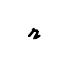
\begin{tikzpicture}[>=round cap]
        \clip (0.085em,-0.1ex) rectangle (0.61em,0.875ex);
        \draw [line width=.2ex, <->, rounded corners=0.13ex] (0.1em,0.1ex) .. controls (0.24em,0.4ex) .. (0.35em,0.8ex) .. controls (0.29em,0.725ex) .. (0.25em,0.6ex) .. controls (0.7em,0.8ex) and (0.08em,-0.4ex) .. (0.55em,0.25ex);
    \end{tikzpicture}
}
}
\newcommand{\hrc}{\hat{\brc}}
%%%%%%%%%%%%%%%%%%%%%%%%%%%%%%%%%%%%%%%%%%%%%%%%%%%%%%%%%%%%%%%%%%%%%%%%%%%%%%%%%%%%%%%%%%%%%%


\begin{document}
	\begin{center}
		\textbf{\Large{PHY250: Formulas and Notes}}\\
		\textit{Kuzma Cosmos (2022)}
	\end{center}
	\textit{This document is for reviewing references and is based on Prof Grizouard's lecture notes and Griffiths E\ \&\ M Textbook. Use in the course only.}
	\tableofcontents
	\newpage
	
\section{Vector Calculus}
	\subsection{Dot product, Cross product, Triple Product}
	The \textbf{dot product} of two vectors \(\overrightarrow{a},\ \overrightarrow{b}\) is defined as:
	\begin{equation}
		\overrightarrow{a}\cdot \overrightarrow{b}=||\overrightarrow{a}||||\overrightarrow{b}||\cos\theta
	\end{equation}
	Algebraically, if \(\overrightarrow{a}=<a_1, a_2, ..., a_n>,\overrightarrow{b}=<b_1, b_2,..., b_n>\), then:
	
	\[\overrightarrow{a}\cdot \overrightarrow{b}=\sum_{i=1}^n a_ib_i\]
	
	\noindent The \textbf{cross product} of two vectors (usually in \(\mathbb{R}^3\) is defined as:
	\begin{equation}
		\overrightarrow{a}\times \overrightarrow {b}=||\overrightarrow{a}||||\overrightarrow{b}||\sin\theta\ \hat{n}
	\end{equation}
	where \(\hat{n}\) is the unit vector pointing to direction of cross product vector. And algebraically:
	\[\overrightarrow{a}\times \overrightarrow{b}=\begin{vmatrix} i& j &k \\ a_1 &a_2  &a_3 \\b_1  &b_2  &b_3 \end{vmatrix}\]
	
	\noindent Notice that, \(\overrightarrow{a}\times \overrightarrow{b}=-\overrightarrow{b}\times \overrightarrow{a}\).
	
	\noindent Some properties of \textbf{Triple products} (Cross-Cross, Cross-Dot, Dot-Cross):
	\begin{itemize}
		\item \(\textbf{A}\cdot (\textbf{B}\times \textbf{C})= \textbf{B}\cdot (\textbf{C}\times \textbf{A})=\textbf{C}\cdot (\textbf{A}\times \textbf{B})\)
		\item \(\textbf{A}\cdot(\textbf{B}\times \textbf{C})=(\textbf{A}\times \textbf{B})\cdot \textbf{C}\)
		\item \(\textbf{A}\times(\textbf{B}\times \textbf{C})=\textbf{B}(\textbf{A}\cdot \textbf{C})-\textbf{C}(\textbf{A}\cdot \textbf{B})\), \textit{BAC-CAB Rule}
		\item From BAC-CAB we can derive that \(\textbf{A}\times(\textbf{B}\times \textbf{C})+\textbf{B}\times(\textbf{C}\times \textbf{A})+\textbf{C}\times(\textbf{A}\times \textbf{B})=\textbf{0}\)
	\end{itemize}
	\subsection{Differential Calculus}
	\subsubsection{Gradient vector}
	In the 3D coordinate system, we first define a point \(\overrightarrow{r}=(x,y,z)\). Then its infinitesimal displacement vector from \((x,y,z)\) to \((x+dx, y+dy, z+dz)\) will be:
	\begin{equation}
		d\overrightarrow{r}=dx\hat{x}+dy\hat{y}+dz\hat{z}
	\end{equation}
	
	\noindent Suppose we have a function of temperature with respect to position in 3D:
	\[T(\overrightarrow{r})=T(x,y,z)\]
	When we move from \(\overrightarrow{r}\) to \(\overrightarrow{r}+d\overrightarrow{r}\), we get the infinitesimal of temperature \(dT\):
	\[dT=(\frac{\partial T}{\partial x})dx+(\frac{\partial T}{\partial y})dy+(\frac{\partial T}{\partial z})dz\]
	We relate the above equation to the vector, given that the dot product of two identical unit vector equals to 1:
	\begin{eqnarray*}
		dT &=& \left(\frac{\partial T}{\partial x}\hat x+\frac{\partial T}{\partial y}\hat y+\frac{\partial T}{\partial z}\hat z\right)\cdot (dx\hat x+ dy\hat y+dz\hat z)\\
		&=& \overrightarrow{\nabla} T \cdot d\overrightarrow{r}
	\end{eqnarray*}
	The vector \(\nabla T\) is a vector quantity, which is called \textbf{gradient vector} of function \textit{T}. Geometrically, the gradient vector \(\nabla T\) points to the direction of \textbf{maximum increase} in temperature.\\
	
	\noindent \textit{Meaning of maximum increase?}\\
	\noindent Consider a contour map showing an inclined plane, where these lines are curves of function \(z=h(x,y)\). Suppose we stand on 60m contour line, and we want to move to one direction with highest increase of altitude. Then what will be this direction?
	\begin{figure}[h]
		\centering
		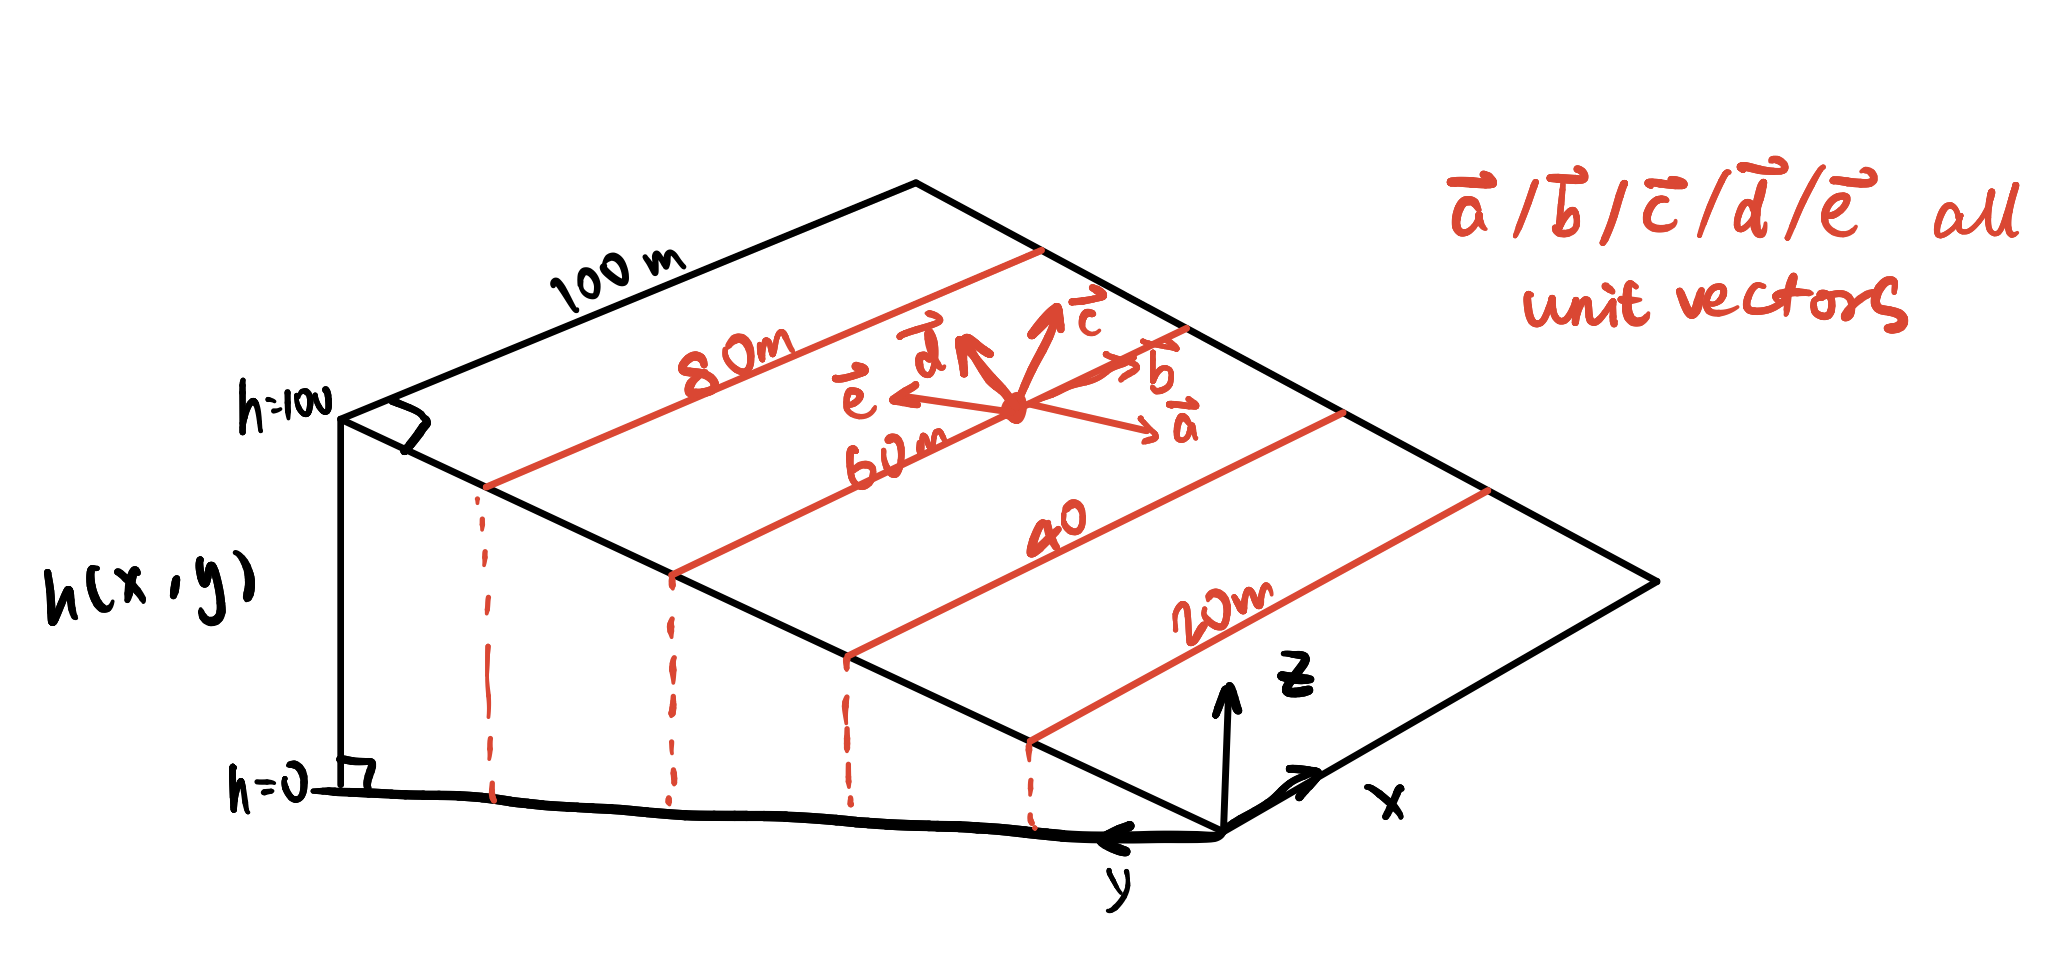
\includegraphics[width=11cm]{gradient_meaning.png}
		\label{fig:1}
		\caption{Meaning of gradient vector}
	\end{figure}
	In other words, we need a vector such that it can move from 60m to 80m height with shortest distance. Among these unit vectors, \(\overrightarrow{d}\) is the desired one for approaching this, because it's perpendicular to all contour lines, indicating "shortest distance between contour lines". This vector \(\overrightarrow{d}\) is the gradient vector \(\overrightarrow{\nabla}\) we want. Notice that vector \(\overrightarrow{b}\) is parallel to the contour lines, and actually in the reality this will be the directional derivative of this contour. Therefore, we have concluded a very important property of gradient:
	\begin{center}
		\textit{\hl{Gradient vector at one point is always perpendicular to directional derivative vector.}}
	\end{center}
	
	\subsubsection{Divergence and Curl}
	Consider a black hole and sun: while the sun emits EMR (such as visible light, and UV radiation), the black hole absorbs all particles, including the EMR like visible light, from its surrounding environments. \\
	
	\noindent We therefore define the term \textbf{divergence}: geometrically speaking, the divergence is a measure of how much the vector $\overrightarrow{v}$ spreads out/diverge from a given point. We further define the vectors which converge into one point have negative divergence. So based on the above example, radiation vectors near a black hole have \textit{negative} divergence, and those near stars have \textit{positive} divergence.\\
	
	\noindent Algebraically, \hl{the \textbf{divergence} is defined as dot product of Del and vector}:
	\begin{equation}
		\mathrm{Div(\textbf{v})}=\nabla\cdot\textbf{v} = \frac{\partial v_x}{\partial x}+\frac{\partial v_y}{\partial y}+\frac{\partial v_z}{\partial z}
	\end{equation}
	Notice that divergence is a scalar value. Fig 1.18 of Griffith textbook show three vector fields: the (a) has a source point emitting vectors,  therefore the divergence is positive. In part (b) there is no difference in each of the vector and therefore has zero divergence. In part (c), instead of a point source, we now have a line source emitting the vectors with increasing lengths, therefore this vector function has positive divergence.
	\begin{figure}[h]
		\centering
		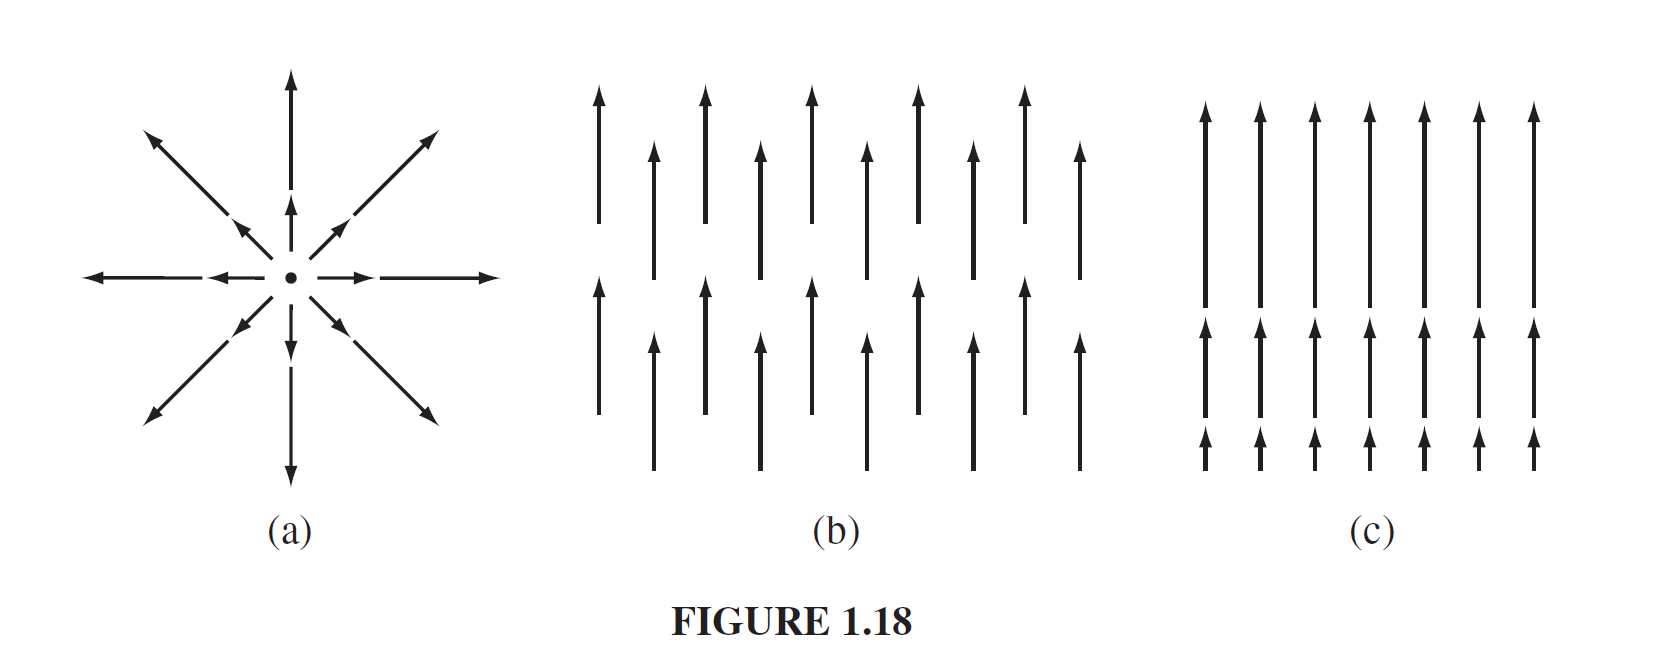
\includegraphics[width=11cm]{divergence.png}
		\caption{Fig 1.18 from Griffith}
		\label{fig:1.18}
	\end{figure}
	
	\noindent \hl{The \textbf{curl} of vectors is defined as cross product of gradient and vectors}:
	\begin{equation}
		\mathrm{Curl(\textbf{v})} = \nabla\times \textbf{v} = \begin{vmatrix} \hat{x}& \hat{y} &\hat{z} \\ \partial/\partial x & \partial/\partial y  &\partial/\partial z \\v_x  &v_y  &v_z \end{vmatrix}
	\end{equation}
	Expanding this equation we have:
	\[\nabla\times \textbf{v}=\hat{x}\left(\frac{\partial v_z}{\partial y}-\frac{\partial v_y}{\partial z}\right) +\hat{y}\left(\frac{\partial v_x}{\partial z}-\frac{\partial v_z}{\partial x}\right)+\hat{z}\left(\frac{\partial v_y}{\partial x}-\frac{\partial v_x}{\partial y}\right)\]
	Notice that, the curl of vector function is still a vector quantity. Geometrically, the curl of vector shows how this vector swirl around one point. For example, all three vector fields in Griffith Fig \ref{fig:1.18} have zero curls since all these vectors don't swirl around any points. However, in Griffith Fig 1.19, both vector functions have nonzero curls, and they both point to the \(\hat{z}\) direction.
	\begin{figure}[ht!]
		\centering
		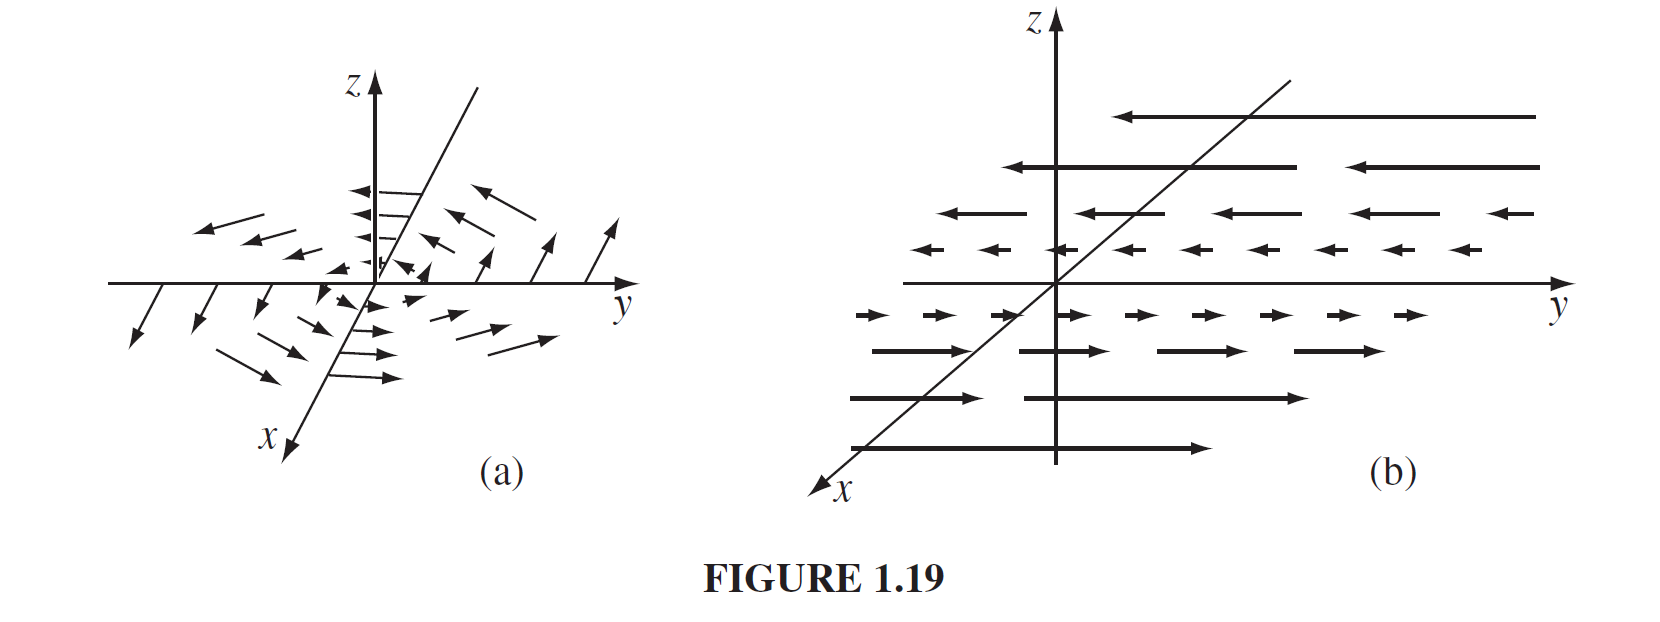
\includegraphics[height=3.2cm]{curl.png}
		\caption{Fig 1.19 from Griffith: notice that both vector fields have non-zero curls }
		\label{fig:1.19}
	\end{figure}
	\subsubsection{Product rules for gradient}
	\begin{itemize}
		\item \(\nabla (f+g)=\nabla f+\nabla g\)
		\item \(\nabla\cdot(\textbf{A}+\textbf{B})=(\nabla\cdot \textbf{A})+(\nabla \cdot \textbf{B})\) (similar for cross product)
		\item \(\nabla\cdot  (k\textbf{A})=k(\nabla\cdot \textbf{A})\) (similar for cross product)
		\item Two rules for gradient:
		\subitem \(\nabla(fg)=f\nabla g+g\nabla f\)
		\subitem \(\nabla(\textbf{A}\cdot \textbf{B})=\textbf{A}\times (\nabla \times \textbf{B})+\textbf{B}\times (\nabla \times \textbf{A})+(\textbf{A}\cdot \nabla)\textbf{B}+(\textbf{B}\cdot \nabla)\textbf{A}\)
		\item Two rules for divergence:
		\subitem \(\nabla \cdot (f\textbf{A})=f(\nabla \cdot \textbf{A})+\textbf{A}\cdot (\nabla f)\)
		\subitem \(\nabla \cdot (\textbf{A}\times \textbf{B})=\textbf{B}\cdot(\nabla \times \textbf{A})-\textbf{A}\cdot (\nabla\times \textbf{B})\)
		\item Two rules for curls:
		\subitem \(\nabla \times (f\textbf{A})=f(\nabla \times \textbf{A})-\textbf{A}\times \nabla f\)
		\subitem \(\nabla \times(\textbf{A}\times \textbf{B})=(\textbf{B}\cdot \nabla)\textbf{A}-(\textbf{A}\cdot \nabla)\textbf{B}+\textbf{A}(\nabla \cdot \textbf{B})-\textbf{B}(\nabla\cdot \textbf{A})\) (\textit{Proof: see PHY250 TUT1/TODO: transfer to this doc})
	\end{itemize}
	
	\subsection{$\cancel{\textrm{Double Del}}$ Second derivatives}
	\begin{itemize}
		\item Gradient derivatives (\(\nabla f\))':
		\subitem a) Divergence of gradient of a scalar function:
		\[\nabla \cdot (\nabla T)=\nabla^2T = \frac{\partial ^2T}{\partial x^2}+\frac{\partial^2 T}{\partial y^2}+\frac{\partial^2 T}{\partial z^2}\]
		where \(\nabla^2 T\) is called \textbf{Laplacian} of \textit{T}
		\subitem b) The Laplacian of a vector function \textbf{v}:
		\[\nabla^2\textbf{v}=(\nabla^2 v_x)\hat{x}+(\nabla^2 v_y)\hat{y}+(\nabla^2 v_z)\hat{z}\]
		which means we need to evaluate the Laplacian three times, each time for each component of vector function \textbf{v}.
		\subitem c) Curl of gradient: \(\nabla\times (\nabla T)\), always \textbf{zero}.
		\item Divergence derivatives (\(\nabla \cdot \textbf{v}\))':
		\subitem a) Gradient of divergence: \(\nabla(\nabla\cdot \textbf{v})\), this seldom appears in physical applications. Differentiate from the Laplacian of vector:
		\[\nabla^2 \textbf{v}=(\nabla \cdot \nabla \textbf{v})\neq\nabla(\nabla \cdot \textbf{v})\]
		\subitem b) Divergence of divergence: \textbf{Undefined} because divergence is scalar instead of vector.
		\subitem c) Curl of divergence: \textbf{Undefined} because divergence is scalar instead of vector.
		\item Curl derivatives (\(\nabla \times \textbf{v}\))':
		\subitem a) Divergence of curl: \(\nabla \cdot (\nabla \times \textbf{v})\), always \textbf{zero}.
		\[\nabla \cdot (\nabla \times \textbf{v})=0\]
		\subitem b) Curl of curl: \(\nabla \times(\nabla\times \textbf{v})\)
		\[\nabla \times(\nabla\times \textbf{v})=\nabla(\nabla \cdot \textbf{v})-\nabla^2\textbf{v}\]
	\end{itemize}
	
	
	\subsection{Vector Integrals}
	Recall from year 1 calculus class:
	\begin{itemize}
		\item We denote \(\frac{df}{dx}\) to show the derivative of function \textit{f} w.r.t. \textit{x}, in geometry this means how fast function \textit{f} varies.
		\item We do anti-derivatives of function's derivative to get its original function expression, which is called "indefinite integral", and by Fundamental Theorem of Calculus, we define the definite integral to the difference of functions evaluated at two bounds:
		\[\int \left(\frac{df}{dx}\right)dx=f(x)+C\]
		\[\int_{a}^{b}\left(\frac{df}{dx}\right)dx=f(b)-f(a)\]
		\item From now on, we will focus on integral calculus on vector functions.
	\end{itemize}
	There are three different types of vector integrals: line integral, surface integral and volume integral.
	
	\subsubsection{Line integral}
	\begin{figure}[ht]
		\centering
		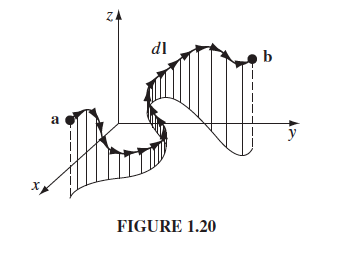
\includegraphics[height = 5cm]{lineintegral.png}
		\label{fig:1.20}
	\end{figure}
	\noindent This is very similar to the definite integral, but we use vectors instead of scalars:
	\begin{equation}
		\int_{\overrightarrow{a}}^{\overrightarrow{b}}\overrightarrow{v}\cdot d\overrightarrow{l}=\int_{\overrightarrow{a}}^{\overrightarrow{b}}v_xdx+v_ydy+v_zdz
	\end{equation}
	
	where \(d\overrightarrow{l}=dx\hat{x}+dy\hat{y}+dz\hat{z}\)\\
	
	\noindent If \(\overrightarrow{a}=\overrightarrow{b}\), the path will be closed and we will put a circle on the integral notation, where \(\mathcal{P}\) is perimeter:
	\[\oint_\mathcal{P}\overrightarrow{v}\cdot d\overrightarrow{l} \]
	To calculate closed line integral, divide the whole perimeter into some pieces and integrate w.r.t them, and then add these integral values up.
	
	\subsubsection{Surface integral}
	\begin{figure}[ht]
		\centering
		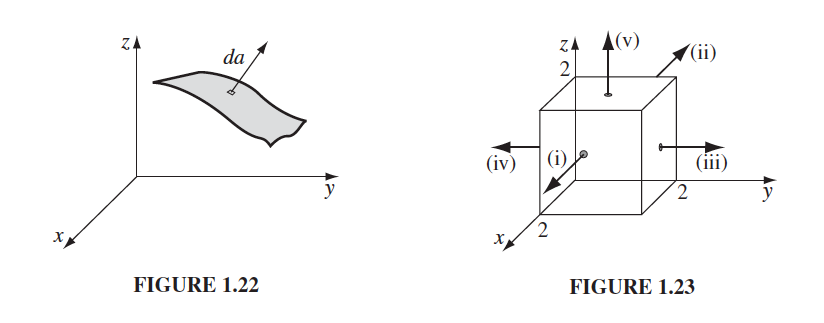
\includegraphics[height = 6cm]{surfaceintegral.png}
		\label{fig: 1.22/23}
	\end{figure}
	\noindent The surface integral is defined as:
	\begin{equation}
		\iint_\mathcal{S} \overrightarrow{v} \cdot d\overrightarrow{a}
	\end{equation}
	
	where \(d\overrightarrow{a}\) is the area element, \textbf{and by convention, it always points outward of surface, which means "flux" of this infinitesimal surface}. And surface integral evaluates the total flux of vector function passing through the surface.\\
	
	\noindent Therefore, if \(\overrightarrow{v}\parallel d\overrightarrow{a}\), which means vector \(\overrightarrow{v}\) the flux of surface would reach maximum, then:
	\[\overrightarrow{v}\cdot d\overrightarrow{a}=vda\]
	
	If \(\overrightarrow{v}\perp d\overrightarrow{a}\), which means vector \(\overrightarrow{v}\) will be parallel to the surface, hence there will be no flux on the surface:
	\[\overrightarrow{v}\cdot d\overrightarrow{a}=0\]
	
	If the surface \(\mathcal{S}\) is closed, then we put the circle on the double integral sign to represent closed surface integral:
	\[\oiint_\mathcal{S} \overrightarrow{v} \cdot d\overrightarrow{a}\]
	
	To evaluate the closed surface integral, we also need to separate the surface into some pieces, evaluating the surface integrals individually and add them up. (Fig 1.23, and see Ex 1.7 on Griffiths)
	\subsubsection{Volume integral}
	Similar to the surface integral, volume integral is defined as:
	\begin{equation}
		\iiint_\mathcal{V} T d\tau
	\end{equation}
	where \(d\tau \) is the infinitesimal solid volume, i.e. \(d\tau=dxdydz\). For a vector function \(\textbf{v}\), the equation becomes:
	\[\iiint_\mathcal{V}\textbf{v} d\tau=\hat{x}\iiint_\mathcal{V} v_xd\tau+\hat{y}\iiint_\mathcal{V}v_yd\tau+\hat{z}\iiint_\mathcal{V}v_zd\tau\]
	
	
	\subsubsection{Fundamental theorem of vector calculus (Lite)}
	There are three types of "fundamental theorems" in vector calculus:
	\begin{enumerate}
		\item Fundamental theorem for gradients: recall that \(dT=(\nabla T)\cdot d\overrightarrow{l}\), then:
		\begin{equation}
		    \int_{\overrightarrow{a}}^{\overrightarrow{b}}dT=T(\overrightarrow{b})-T(\overrightarrow{a})=\int_{\overrightarrow{a}}^{\overrightarrow{b}}(\nabla T)\cdot d\overrightarrow{l}
		    \label{eq:9}
		\end{equation}
		
		\item Fundamental theorem for divergences ("Divergence theorem", "Green's theorem"): suppose a solid \(\mathcal{V}\) is bounded by surface \(\mathcal{S}\), then:
		\begin{equation}
		    \iiint_{\mathcal{V}}(\nabla \cdot \overrightarrow{v})d\tau=\oiint_{\mathcal{S}}\overrightarrow{v}\cdot d\overrightarrow{a}
		    \label{eq:10}
		\end{equation}
		
		\item Fundamental theorem for curl ("Stokes' theorem"): suppose we have a surface \(\mathcal{S}\) where \(\mathcal{P}\) is its exact perimeter of \(\mathcal{S}\). Then the Stokes' theorem states that:
		\begin{equation}
		    \iint_{\mathcal{S}}(\nabla\times\overrightarrow{v})\cdot d\overrightarrow{a}=\oint_{\mathcal{P}}\overrightarrow{v}\cdot d\overrightarrow{l}
		    \label{eq:11}
		\end{equation}
		
		where \((\nabla \times \overrightarrow{v})\cdot d\overrightarrow{a}\) means the local spin density across \(d\overrightarrow{a}\) and its integral will be the local flux of "spin" (curl) across surface \(\mathcal{S}\).\\
		
		And now we circulate around perimeter \(\mathcal{P}\), if there is total net spin, then \(\overrightarrow{v}\cdot d\overrightarrow{l}>0\implies\oint\overrightarrow{v}\cdot d\overrightarrow{l}>0\). To determine direction of circulation, use right hand screw law oriented by direction of $d\overrightarrow{a}$.
	\end{enumerate}
	
	
	\subsection{Different coordinate systems}
	We mainly focus on two types of coordinate system in \(\mathbb{R}^3\) space: cylindrical coordinates and spherical coordinates.
	\subsubsection{Cylindrical coordinates: \((x,y,z)\rightarrow(r,\phi,z)\)}
	\begin{figure}[ht]
		\centering
		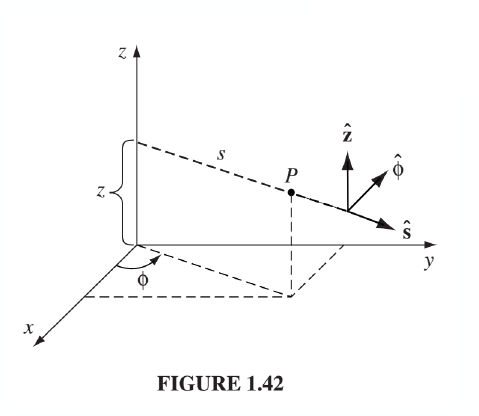
\includegraphics[width = 10cm]{250-Revision/cylindrical.png}
		\caption{Cylindrical coordinates}
		\label{fig:cylindrical}
	\end{figure}
	This is actually the combination of polar coordinates with $z$ axis, where the radial length from origin is $r$ (or $s$ in the above figure), angle between x-axis and the radial line \(\phi\) and $z$ value.
	
	For the unit vector directions of the component vectors, $\hat{s}$ points outward and parallel to radial line, $\hat{\phi}$ is parallel to $xy$-plane and is perpendicular to $\hat{s}$, and $\hat{z}$ is certainly pointing to +$z$ direction as in the Cartesian coordinate.\\
	
	\noindent Some properties:
	\begin{itemize}
		\item Conversion between cylindrical and Cartesian coordinate components:
		\begin{eqnarray*}
			x &=& s\cos\phi\\
			y &=& s\sin\phi\\
			z &=& z
		\end{eqnarray*}
		\item Conversion between cylindrical and Cartesian basis unit vectors 
		\[\overrightarrow{P}=P_s\hat{s}+P_\phi\hat{\phi}+P_z\hat{z}\]
		\begin{eqnarray*}
			\hat{s} &=& \cos\phi\hat{x} + \sin\phi\hat{y}\\
			\hat{\phi} &=& -\sin\phi\hat{x} + \cos\phi\hat{y}\\
			\hat{z} &=& \hat{z}
		\end{eqnarray*}
		\item Infinitesimal displacement vector:
		\begin{eqnarray*}
			d\overrightarrow{l} &=& dl_s\hat{s}+dl_\phi\hat{\phi}+dl_z\hat{z}\\
			&=& ds\hat{s}+sd\phi\hat{\phi}+dz\hat{z}
		\end{eqnarray*}
		
		\item Volume/Area elements:
		\begin{itemize}
			\item Volume element: \(d\tau=sdsd\phi dz\)
			\item Area element in $s$ direction: \(d\overrightarrow{a}=sd\phi dz\hat{s}\)
			\item Area element in $z$ direction: \(d\overrightarrow{a}=sd\phi dz\hat{z}\)
		\end{itemize}
		\item Derivatives:
		\begin{eqnarray*}
			\nabla T &=& \frac{\partial T}{\partial s}\hat{s}+\frac{1}{s}\frac{\partial T}{\partial \phi}\hat{\phi}+\frac{\partial T}{\partial z}\hat{z}\\
			\nabla \cdot \overrightarrow{v} &=& \frac{1}{s}\frac{\partial sv_s}{\partial s} +\frac{1}{s}\frac{\partial v_\phi}{\partial \phi}+\frac{\partial v_z}{\partial z}\\
			\nabla \times \overrightarrow{v} &=& \hat{s}\left[\frac{1}{s}\frac{\partial v_z}{\partial \phi}-\frac{\partial v_\phi}{\partial z}\right]+\hat{\phi}\left[\frac{\partial v_s}{\partial z}-\frac{\partial v_z}{\partial s}\right]+\hat{z}\frac{1}{s}\left[\frac{\partial (sv_\phi)}{\partial s}-\frac{\partial v_s}{\partial \phi}\right]\\
			\nabla^2T &=& \frac{1}{s}\frac{\partial}{\partial s}\left(s\frac{\partial T}{\partial s}\right) + \frac{1}{s^2}\frac{\partial^2 T}{\partial\phi^2}+\frac{\partial^2T}{\partial z^2}
		\end{eqnarray*}
	\end{itemize}
	
	\subsubsection{Spherical coordinates: \((x,y,z)\rightarrow(r,\theta,\phi)\)}
	
	\begin{figure}[ht]
		\centering
		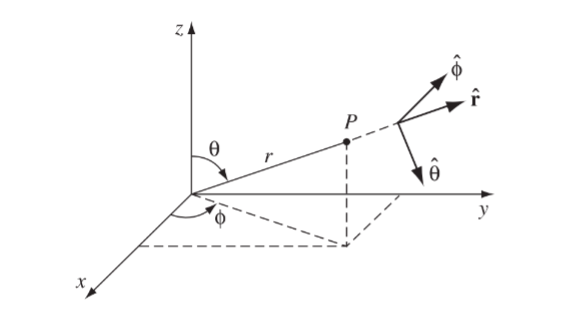
\includegraphics[width=10cm]{250-Revision/spherical.png}
		\caption{Spherical coordinates}
		\label{fig:spherical}
	\end{figure}
	$\theta$ angle measured from $z$ axis, $r$ is the radial distance, and angle $\phi$ is measured from $x$ axis.\\
	
	Some properties:
	\begin{itemize}
		\item Basis vectors:
		\subitem $\hat{r}$ points radially outward
		\subitem $\hat{\theta}$ perpendicular to $\hat{r}$ but with $+\theta$ direction
		\subitem $\hat{\phi}$ perpendicular to $\hat{r}$ but with $+\phi$ direction
		
		\item Conversion between spherical and Cartesian basis vectors/coordinates:
		\subitem \(P=P_r\hat{r}+P_\theta\hat{\theta}+P_\phi\hat{\phi}\)
		\subitem \(x = r\sin\theta\cos\phi\)
		\subitem \(y=r\sin\theta\sin\phi\)
		\subitem \(z=r\cos\theta\)
		\subitem \(\hat{r}=\sin\theta\cos\phi\hat{x}+\sin\theta\sin\phi\hat{y}+\cos\theta\hat{z}\)
		\subitem \(\hat{\theta}=\cos\theta\cos\phi\hat{x}+\cos\theta\sin\phi\hat{y}-\sin\theta\hat{z}\)
		\subitem \(\hat{\phi}=-\sin\phi\hat{x}+\cos\phi\hat{y}\)
		
		\item Infinitesimal displacement vector:
		\begin{eqnarray*}
			d\overrightarrow{l} &=& dl_r\hat{r}+dl_\theta\hat{\theta}+dl_\phi\hat{\phi}\\
			&=& dr\hat{r}+rd\theta \hat{\theta} + r\sin\theta d\phi\hat{\phi}
		\end{eqnarray*}
		\begin{figure}[h]
			\centering
			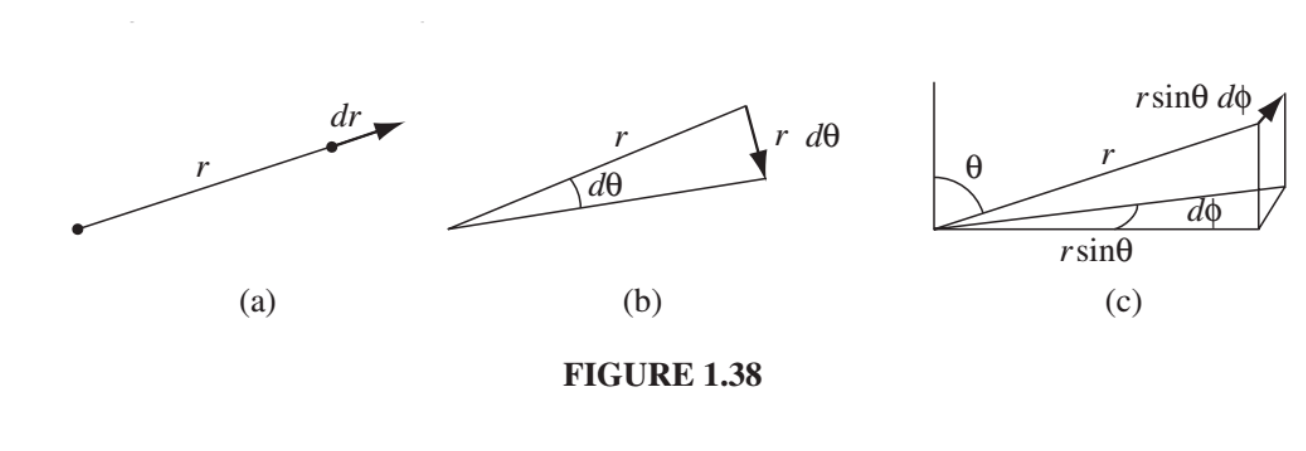
\includegraphics[width=12cm]{250-Revision/spheric-dl.png}
			\caption{Infinitesimal displacement vector decomposition}
			\label{fig:spheric-dl}
		\end{figure}
		
		\item Area element:
		\begin{eqnarray*}
			d\overrightarrow{a} &=& da\hat{r}\\
			&=& dl_\theta dl_\phi \hat{r} \\
			&=& rd\theta r\sin\theta d\phi\hat{r}\\
			&=& r^2\sin\theta d\theta d\phi \hat{r}
		\end{eqnarray*}
		\begin{figure}[ht]
			\centering
			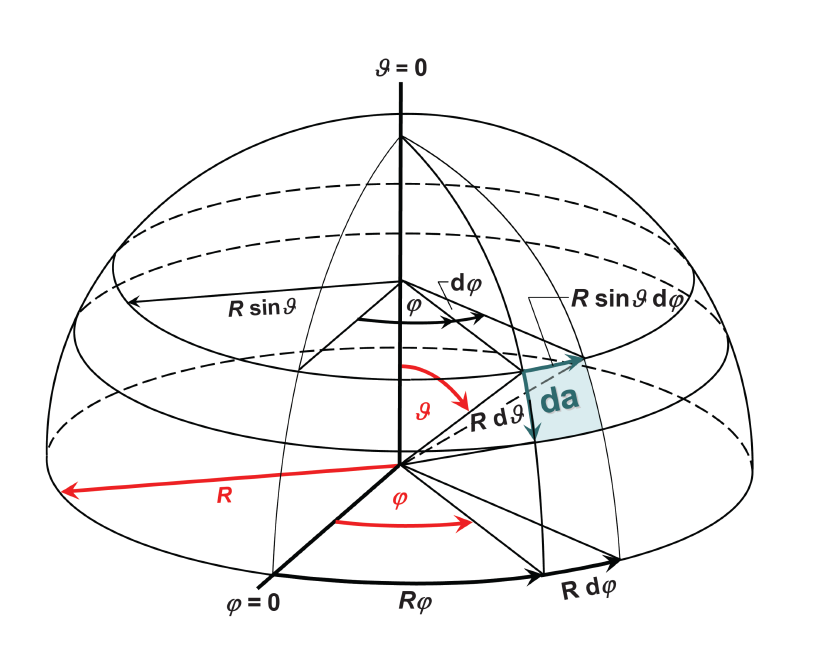
\includegraphics[height=5cm]{250-Revision/spherical-da.png}
			\caption{Area element}
			\label{fig:spherical-da}
		\end{figure}
		
		\item Volume element:
		\[d\tau =r^2\sin\theta d\theta d\phi dr\]
		\begin{figure}[h]
			\centering
			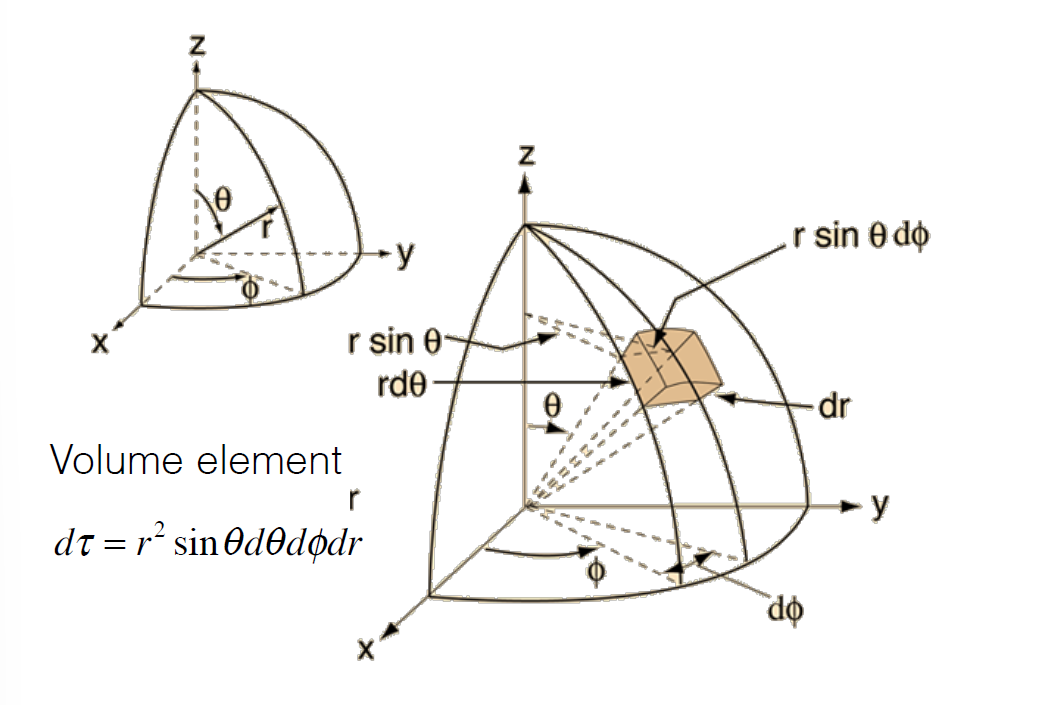
\includegraphics[height=5cm]{250-Revision/spherical-dtau.png}
			\caption{Volume element}
			\label{fig:spherical-dtau}
		\end{figure}
		
		\item Derivatives
		\begin{eqnarray*}
			\nabla T &=& \frac{\partial T}{\partial r}\hat{r} + \frac{1}{r}\frac{\partial T}{\partial \theta}\hat{\theta} + \frac{1}{r\sin\theta}\frac{\partial T}{\partial \phi}\hat{\phi}\\
			\nabla \cdot \overrightarrow{v} &=& \frac{1}{r^2}\frac{\partial}{\partial r}(r^2v_r) +\frac{1}{r\sin\theta}\frac{\partial}{\partial\theta}(\sin\theta v_\theta)+\frac{1}{r\sin\theta}\frac{\partial v_\phi}{\partial \phi}\\
			\nabla \times \overrightarrow{v} &=& \frac{1}{r\sin\theta}\left[\frac{\partial}{\partial \theta}(\sin\theta v_\phi)-\frac{\partial v_\theta}{\partial \phi}\right]\hat{r}+\\
			& & \frac{1}{r}\left[\frac{1}{\sin\theta}\frac{\partial v_r}{\partial \phi}-\frac{\partial}{\partial r}(rv_\phi)\right]\hat{\theta}+\\
			& & \frac{1}{r}\left[\frac{\partial}{\partial r}(rv_\theta)-\frac{\partial v_r}{\partial\theta}\right]\hat{\phi}\\
			\nabla^2T &=& \frac{1}{r^2}\frac{\partial}{\partial r}\left(r^2\frac{\partial T}{\partial r}\right) + \frac{1}{r^2\sin\theta}\frac{\partial}{\partial \theta}\left(\sin\theta\frac{\partial T}{\partial \theta}\right) +\frac{1}{r^2\sin^2\theta}\frac{\partial^2T}{\partial\phi^2} 
		\end{eqnarray*}
		
	\end{itemize}
	
	
	
	\subsection{Dirac Delta function (Lecture 5)}
	Here is a vector function:
	\[\overrightarrow{v} =\frac{\hat{r}}{r^2}\]
	Suppose we want to evaluate the divergence and test the Divergence Theorem using this vector function... Here we go:\\
	
	\noindent According to Equation \ref{eq:10}:
	\[\iiint (\overrightarrow{\nabla}\cdot (\frac{\hat{r}}{r^2}))d\tau=\oiint \frac{\hat{r}\cdot d\overrightarrow{a}}{r^2}\]
	
    \begin{itemize}
	    \item RHS: This closed surface integral tells the flux of \(\hat{r}/r^2\) across a sphere of radius $R$:
	    \[d\overrightarrow{a}=dl_\theta dl_\phi \hat{r}=r^2\sin\theta d\theta d\phi \hat{r}\]
	    \[\overrightarrow{v}\cdot d\overrightarrow{a}=\sin\theta d\theta d\phi\]
	    \[\oiint = \int_0^{2\pi}d\phi\int_0^{\pi}\sin\theta d\theta =2\pi(-\cos\pi+\cos (1))=4\pi\]
	    
	    \item LHS:
	    \[\nabla \cdot (\frac{\hat{r}}{r^2})=\frac{1}{r^2}\frac{\partial}{\partial r}(r^2v_r)=\frac{1}{r^2}\frac{\partial}{\partial r}(r^2\cdot\frac{1}{r^2})=0\]
	    \[\iiint (\nabla\cdot \overrightarrow{v})d\tau = 0\]
	    However,the expected value of this triple integral is not zero but $4\pi$, something wrong happened here... Actually the problem is from the position where $r=0$: $\nabla\cdot\overrightarrow{v}$ does be zero everywhere except $r=0$. Therefore we need some extra function to handle this special position.
	\end{itemize}
	
	\subsubsection{Dirac Delta distribution in 1D}
	We define a distribution function $\delta(x)$:
	\begin{equation}
	    \delta(x)=\left\{\begin{matrix}
        0\ (x\neq 0)\\ 
        \infty\ (x=0)
    \end{matrix}\right.
	\end{equation}
	And we further define it:
	\[\forall a,b\in \mathbb{R},\ a<0<b\implies  \int_{a}^{b}\delta(x)dx=1\]
	In other words:
	\[\delta(x)=\lim_{a\to 0}\left(\frac{1}{a\sqrt{\pi}}e^{-(x/a)^2}\right)\]
	Some properties of Dirac Delta:
	\begin{itemize}
	    \item \(f(x)\delta(x)=f(0)\delta(x)\) and \(\int_a^bf(x)\delta(x)dx=f(0)\ (a<0<b)\)
	    \item \(\delta(x-a)=\infty\) for $x=a$, \(\delta(x-a)=0\) otherwise
	    \item \(\int_a^bf(x)\delta(x-\alpha)dx=f(\alpha)\ (a<\alpha<b)\)
	    \item \(f(kx)=\frac{1}{|k|}\delta(x)\) (proof: see Textbook p.48-9 Example 1.15)
	\end{itemize}
	
	\subsubsection{Dirac Delta in 3D}
	\begin{equation}
	   \delta^3(\overrightarrow{r}) = \delta(x)\delta(y)\delta(z)
	\end{equation}
	Similar to 1D Dirac Delta, \(\delta^3(\overrightarrow{r})\) is zero everywhere except (0,0,0). And its volume integral will be:
	\begin{equation}
	    \iiint_{\mathbb{R}^3}\delta^3(\overrightarrow{r})d\tau = \int_{-\infty}^{\infty}\int_{-\infty}^{\infty}\int_{-\infty}^{\infty}\delta(x)\delta(y)\delta(z)dxdydz = 1
	\end{equation}
	\begin{equation}
	    \iiint_{\mathbb{R}^3}f(\overrightarrow{r})\delta^3(\overrightarrow{r}-\overrightarrow{\alpha})d\tau = f(\overrightarrow{a})
	\end{equation}
	
	\noindent Back to the original triple integral:
	\[\iiint (\nabla\cdot \frac{\hat{r}}{r^2})d\tau\]
	Since we know that this triple integral should be $4\pi$ according to the RHS of Divergence Theorem, then \(\nabla\cdot (\frac{\hat{r}}{r^2})\) should be 0 everywhere except being $\infty$ at origin.
	\[\nabla\cdot(\frac{\hat{r}}{r^2})=4\pi \delta^3(\overrightarrow{r})\]
	
	
	\subsection{The theory of vector fields - Helmholtz theorem}
	Suppose we have a continuous single variable function $f(x)$, knowing $f(x_0)$ as initial condition, and its derivative $df/dx$. Then we can evaluate the function everywhere according to the fundamental theorem of calculus:
	\[f(x)=f(x_0)+\int_{x_0}^{x}\frac{df}{dx'}(x')dx'\]
    Now, we have a vector field \(\overrightarrow{F}\), and we know its divergence and curl, and some boundary conditions, then can we evaluate \(\overrightarrow{F}\)? YES! By using Helmholtz Theorem. It is not easy to apply this directly, instead we can look for some cases.\\
	
    \begin{itemize}
        \item \textbf{Case 1}: \(\nabla\times \overrightarrow{F}=\overrightarrow{0}\)
        In this case, this field is qualified as "irrotational", according to geometric meaning of curl. Then we have the following theorem:
        \begin{description}
	        \item[THEOREM] $\nabla\times\overrightarrow{F} = \overrightarrow{0}\iff \exists V(x,y,z)$, $\overrightarrow{F}=-\nabla V$
        \end{description}
        where $V$ is called the \textit{scalar potential}, defined up to a constant.
        
        Irrotational fields have the following properties:
        \begin{itemize}
            \item \(\overrightarrow{F}=-\nabla V\)
            \item \(\nabla \times \overrightarrow{F}=\overrightarrow{0}\) 
            \item \(\oint \overrightarrow{F}\cdot d\overrightarrow{l}=0\)
            \item \(\int_{\overrightarrow{a}}^{\overrightarrow{b}}\overrightarrow{F}\cdot d\overrightarrow{l}\) is path-independent. This property and the third one are derived from gradient theorem.
        \end{itemize}
        
        \item \textbf{Case 2:} \(\nabla\cdot \overrightarrow{F}=0\), we say that this field is "solenoidal".Then we have the following theorem:
        \begin{description}
	        \item[THEOREM] $\nabla\cdot\overrightarrow{F} = 0\iff \exists\overrightarrow{A}$, $\overrightarrow{F}=\nabla\times\overrightarrow{A}$
        \end{description}
        where $\overrightarrow{A}$ is called the \textit{vector potential}, defined up to a gradient.
        
        Solenoidal fields have the following properties:
        \begin{itemize}
            \item \(\overrightarrow{\nabla}\cdot\overrightarrow{F}=0\)
            \item \(\overrightarrow{F}=\overrightarrow{\nabla}\times\overrightarrow{A}\)
            \item \(\oiint \overrightarrow{F}\cdot d\overrightarrow{a}=0\) (Stoke's Theorem, and iff first condition is also true)
            \item \(\iint_\mathcal{S}\overrightarrow{F}\cdot d\overrightarrow{a}\) is surface independent (Stoke's Theorem)
        \end{itemize}
    \end{itemize}
	
	\noindent Thus, we can conclude the general case:
	\begin{description}
	    \item [Helmholtz's Theorem] Suppose we have a vector field $\overrightarrow{F}$, and know that its divergence and curl are not zero, then there always exists $V$ and $\overrightarrow{A}$, which approach to zero at infinity, such that
	    \begin{equation}
	        \overrightarrow{F}=-\overrightarrow{\nabla}V+\overrightarrow{\nabla}\times\overrightarrow{A}
	    \end{equation}
	\end{description}
	\newpage
	
	
	\subsection{Appendix I: Proofs of Some Important Properties of Unit 1}
	\begin{enumerate}
		\item \textit{Claim}: The divergence of curl is always zero.\\
		\textbf{Proof}
		\begin{eqnarray*}
			\nabla \cdot (\nabla \times \textbf{v}) &=& \begin{bmatrix}\frac{\partial}{\partial x}\\\frac{\partial}{\partial y} \\\frac{\partial}{\partial z} \end{bmatrix}\cdot \begin{bmatrix}\frac{\partial v_z}{\partial y}-\frac{\partial v_y}{\partial z}\\\frac{\partial v_x}{\partial z}-\frac{\partial v_z}{\partial x}\\\frac{\partial v_y}{\partial x}-\frac{\partial v_x}{\partial y}\end{bmatrix}\\
			&=& \frac{\partial^2v_z}{\partial x\partial y}-\frac{\partial^2 v_y}{\partial x\partial z}+\frac{\partial^2 v_x}{\partial y\partial z}-\frac{\partial^2 v_z}{\partial y\partial x}+\frac{\partial^2 v_y}{\partial z\partial x}-\frac{\partial^2 v_x}{\partial z\partial y}\\
			&=& 0
		\end{eqnarray*}
		\begin{flushright}
			$\blacksquare$
		\end{flushright}
		
		\item \textit{Claim}: \(\nabla \times (\nabla\times \textbf{v})=\nabla (\nabla\cdot \textbf{v})-\nabla^2\textbf{v}\) (Curl of Curl expression, HW1-2)\\
		
		NOTE: to prove this, we need first evaluate the LHS, then evaluate RHS, and compare whether they are equal. If not equal, then there is some algebra mistakes.\\
		
		\textbf{Proof}
		\begin{itemize}
			\item LHS:
			\begin{eqnarray*}
				\nabla \times (\nabla \times \textbf{v}) &=& \nabla \times \begin{bmatrix}\frac{\partial v_z}{\partial y}-\frac{\partial v_y}{\partial z}\\\frac{\partial v_x}{\partial z}-\frac{\partial v_z}{\partial x}\\\frac{\partial v_y}{\partial x}-\frac{\partial v_x}{\partial y}\end{bmatrix}\\
				&=& \begin{vmatrix}
					\hat{x}	& \hat{y} & \hat{z} \\ 
					\frac{\partial}{\partial x}	&\frac{\partial}{\partial y}  & \frac{\partial}{\partial z}\\ 
					\frac{\partial v_z}{\partial y}-\frac{\partial v_y}{\partial z}	&\frac{\partial v_x}{\partial z}-\frac{\partial v_z}{\partial x}  & \frac{\partial v_y}{\partial x}-\frac{\partial v_x}{\partial y}
					
				\end{vmatrix}\\
				&=& \hat{x}\left(\frac{\partial}{\partial y}\left(\frac{\partial v_y}{\partial x}-\frac{\partial v_x}{\partial y}\right)-\frac{\partial}{\partial z}\left(\frac{\partial v_x}{\partial z}-\frac{\partial v_z}{\partial x}\right)\right) +\\
				& & \hat{y}\left(\frac{\partial}{\partial z}\left(\frac{\partial v_z}{\partial y}-\frac{\partial v_y}{\partial z}\right)-\frac{\partial}{\partial x}\left(\frac{\partial v_y}{\partial x}-\frac{\partial v_x}{\partial y}\right)\right) +\\
				& & \hat{z}\left(\frac{\partial}{\partial x}\left(\frac{\partial v_x}{\partial z}-\frac{\partial v_z}{\partial x}\right)-\frac{\partial }{\partial y}\left(
				\frac{\partial v_z}{\partial y}-\frac{\partial v_y}{\partial z}\right)\right)\\
				&=& \hat{x}\left(\frac{\partial^2 v_y}{\partial y\partial x}-\frac{\partial^2 v_x}{\partial y^2}-\frac{\partial^2 v_x}{\partial z^2}+\frac{\partial^2 v_z}{\partial z\partial x}\right) + \\
				& & \hat{y}\left(\frac{\partial^2v_z}{\partial z\partial y}-\frac{\partial^2v_y}{\partial z^2}-\frac{\partial^2v_y}{\partial x^2}+\frac{\partial^2v_x}{\partial x\partial y}\right) + \\
				& & \hat{z}\left(\frac{\partial^2 v_x}{\partial x\partial z}-\frac{\partial^2v_z}{\partial x^2}-\frac{\partial^2v_z}{\partial y^2}+\frac{\partial^2 v_y}{\partial y\partial z}\right)
			\end{eqnarray*}
			\item RHS:
			
			\begin{eqnarray*}
				\nabla (\nabla \cdot \textbf{v}) &=& \nabla (\frac{\partial v_x}{\partial x}+\frac{\partial v_y}{\partial y}+\frac{\partial v_z}{\partial z}) \\
				&=& \hat{x}\frac{\partial}{\partial x}\left(\frac{\partial v_x}{\partial x}+\frac{\partial v_y}{\partial y}+\frac{\partial v_z}{\partial z}\right)+\\
				& &\hat{y}\frac{\partial}{\partial y}\left(\frac{\partial v_x}{\partial x}+\frac{\partial v_y}{\partial y}+\frac{\partial v_z}{\partial z}\right)+\\
				& &\hat{z}\frac{\partial}{\partial z}\left(\frac{\partial v_x}{\partial x}+\frac{\partial v_y}{\partial y}+\frac{\partial v_z}{\partial z}\right)
			\end{eqnarray*}
			
			\begin{eqnarray*}
				\nabla^2\textbf{v} &=& \hat{x}\left(\frac{\partial^2 v_x}{\partial x^2}+\frac{\partial^2 v_x}{\partial y^2}+\frac{\partial^2 v_x}{\partial z^2}\right) + \\
				& & \hat{y}\left(\frac{\partial^2 v_y}{\partial x^2}+\frac{\partial^2 v_y}{\partial y^2}+\frac{\partial^2 v_y}{\partial z^2}\right) + \\
				& & \hat{z}\left(\frac{\partial^2 v_z}{\partial x^2}+\frac{\partial^2 v_z}{\partial y^2}+\frac{\partial^2 v_z}{\partial z^2}\right)
			\end{eqnarray*}
			
			\begin{eqnarray*}
				\nabla (\nabla \cdot \textbf{v}) - \nabla^2\textbf{v} &=& 
				\hat{x}\left(\cancel{\frac{\partial^2 v_x}{\partial x^2}} + \frac{\partial^2 v_y}{\partial x\partial y} + \frac{\partial^2 v_z}{\partial x\partial z} - \cancel{\frac{\partial^2 v_x}{\partial x^2}} -\frac{\partial^2 v_x}{\partial y^2}-\frac{\partial^2 v_x}{\partial z^2} \right) +\\
				& & \hat{y}\left(\frac{\partial^2 v_x}{\partial y\partial x}+\cancel{\frac{\partial^2 v_y}{\partial y^2}}+\frac{\partial^2 v_z}{\partial y\partial z}-\frac{\partial^2 v_y}{\partial x^2}-\cancel{\frac{\partial^2 v_y}{\partial y^2}}-\frac{\partial^2 v_y}{\partial z^2} \right) +\\
				& & \hat{z}\left(\frac{\partial^2 v_x}{\partial z \partial x}+\frac{\partial^2 v_y}{\partial z\partial y} +\cancel{\frac{\partial^2 v_z}{\partial z^2}}-\frac{\partial^2 v_z}{\partial x^2}-\frac{\partial^2 v_z}{\partial y^2}-\cancel{\frac{\partial^2 v_z}{\partial z^2}} \right)
			\end{eqnarray*}
			\item Comparing the items, we found LHS = RHS, and that completes the proof.
			\begin{flushright}
				$\blacksquare$
			\end{flushright}
			
			
		\end{itemize}
	\end{enumerate}
	
\section{Electrostatics}
\subsection{Coulomb's Law and Electric Field}
\subsubsection{Coulomb's Law: general}
    \begin{figure}[ht]
        \centering
        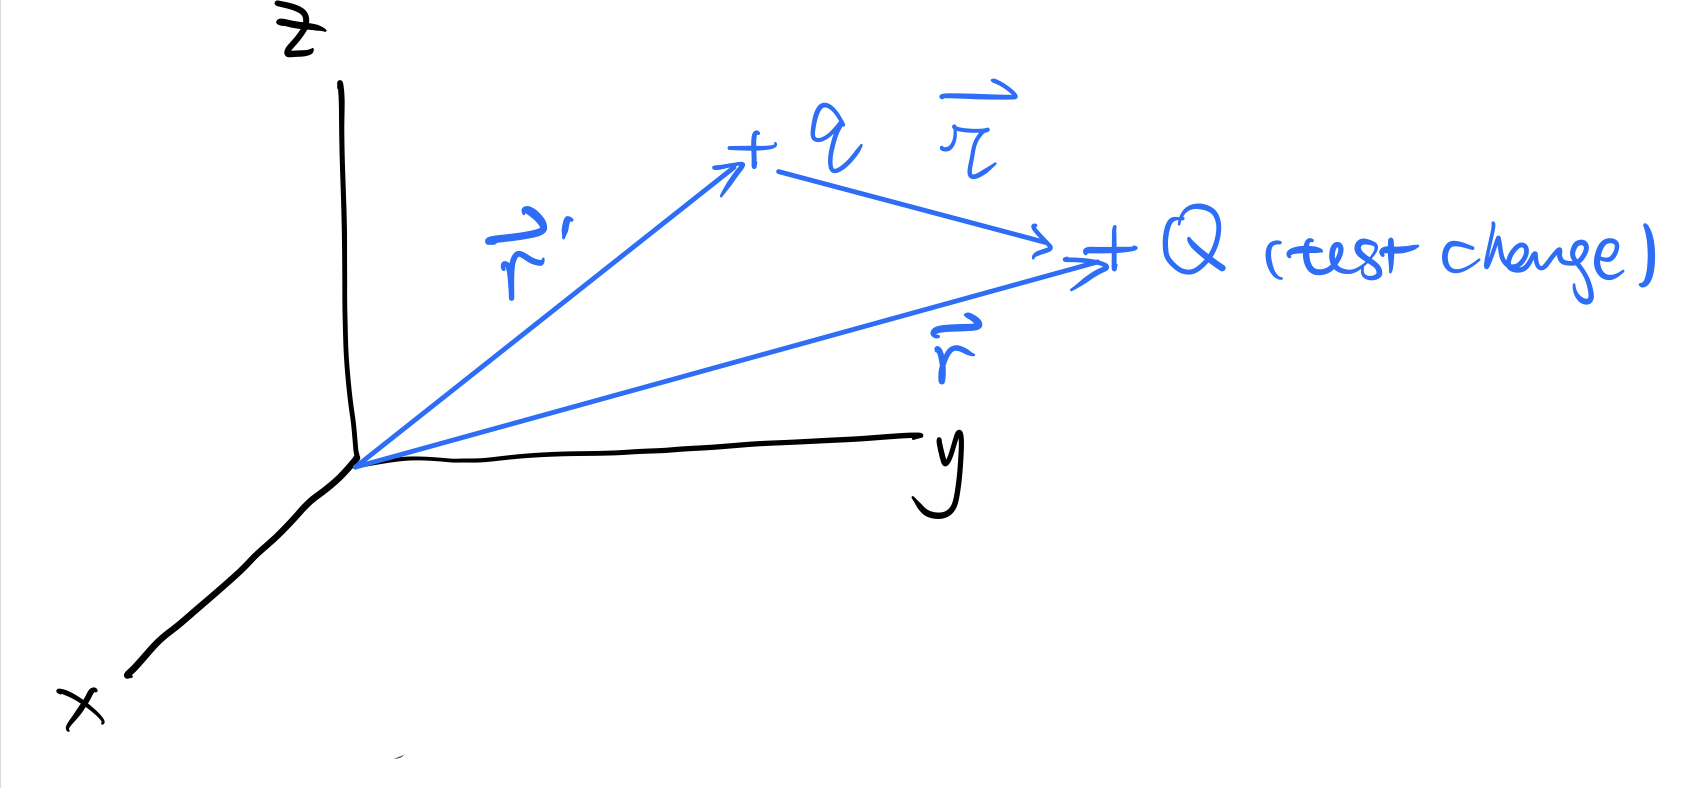
\includegraphics[height=4.6cm]{250-Revision/coulumb.PNG}
        \label{fig:coulumb}
    \end{figure}
    \noindent Suppose there exists a positive charge $+q$, with the distance from the origin $r'$, i.e. defining a vector $\overrightarrow{r'}$ from origin to this charge. We also put a test charge $+Q$, with a vector $\overrightarrow{r}$ from the origin to this test charge. Then the difference vector $\overrightarrow{\rc}=\overrightarrow{r}-\overrightarrow{r'}$.\\
    
    \noindent Then, the electric force of charge $q$ on $Q$ will be
    \begin{equation}
        \overrightarrow{F}=\frac{1}{4\pi\varepsilon_0}\frac{qQ}{\rc^2}\hrc
    \end{equation}
    where
    \begin{itemize}
        \item \(\overrightarrow{F}\) in N (kg m s$^-1$)
        \item $q,Q$ in C (A$\cdot$s)
        \item $\rc$ in m
        \item $\varepsilon_0$ is permittivity of free space, and \(\varepsilon_0=8.85\times 10^{-12}\frac{\mathrm{C}^2}{\mathrm{N\ m^3}}\)
        \item If $q, Q$ have the same size, then the force is repulsive (with +$\hrc$ direction), otherwise it is attractive (with -$\hrc$ direction)
    \end{itemize}
    
    \noindent The electric field of charge $q$ is defined by:
    \begin{equation}
        \overrightarrow{E} = \frac{\overrightarrow{F}}{Q} =\frac{1}{4\pi\varepsilon_0}\frac{q}{\rc^2}\hrc
    \end{equation}
    
    \noindent \textbf{Superposition principle}\\
    \noindent Suppose we have $N$ charges: $q_1, q_2, ..., q_N$, located at $\overrightarrow{r'_1}, \overrightarrow{r'_2},...,\overrightarrow{r'_N}$, then the electric force will be the sum of the total force from each charge:
    \begin{equation}
        \overrightarrow{F}_{tot} = \frac{Q}{4\pi\varepsilon_0} \sum_{i=1}^{N}\frac{q_i}{\rc_i^2}\hrc
    \end{equation}
    \noindent \textit{Exercise: Example 2.1, p.62}
\newpage
\subsubsection{Coulomb's Law: Continuous distribution}
Using the idea of Riemann Sum, we can turn the summation sign into integral.
\begin{itemize}
    \item 1D distribution
    \begin{figure}[h]
        \centering
        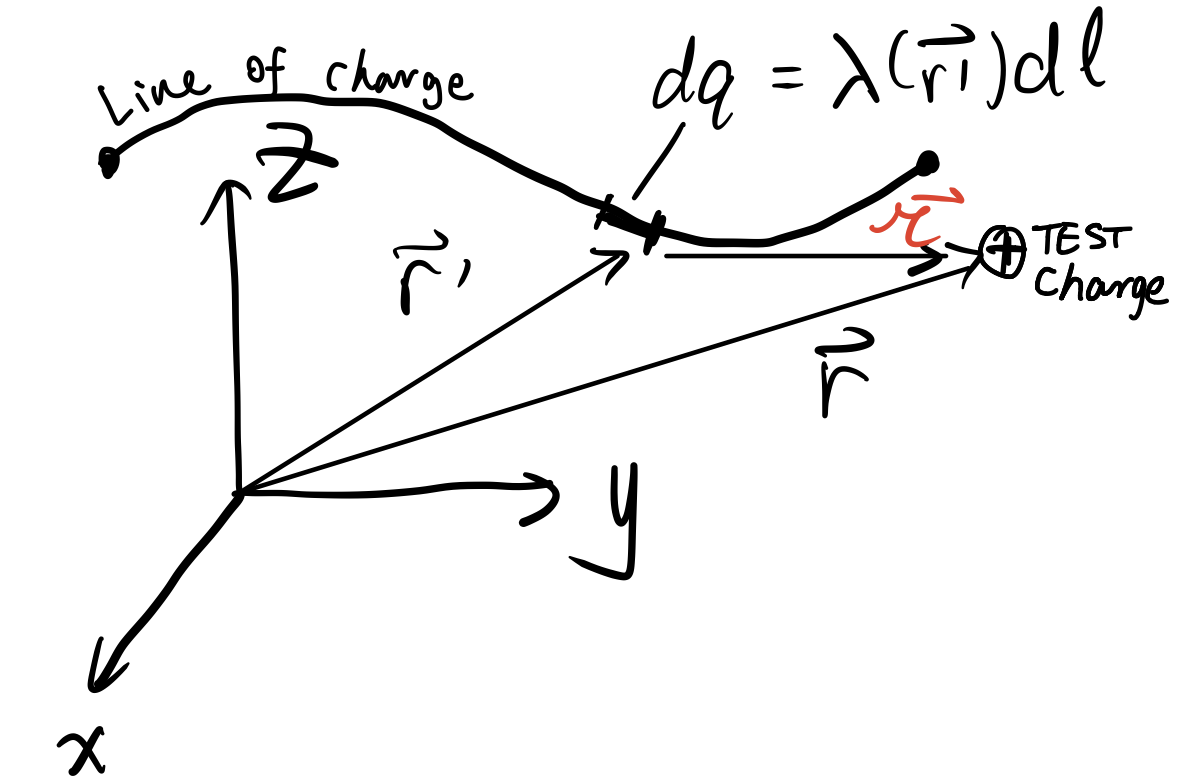
\includegraphics[height=5cm]{250-Revision/1d-charge.png}
        \caption{1D Charge distribution}
        \label{fig:1d-charge}
    \end{figure}\newline
    The infinitesimal charge will be:
    \[dq=\lambda(\overrightarrow{r'}) dl\]
    where $\lambda$ is linear charge density (C/m). Then the electric field will be:
    \begin{equation}
        \overrightarrow{E} = \frac{1}{4\pi\varepsilon_0}\int_{\mathcal{L}}\frac{\lambda(\overrightarrow{r'})\hrc dl}{\rc^2}
    \end{equation}
    where $\mathcal{L}$ is whole line of charge.\\
    \textit{Example: Ex 2.2, p.64 (See Lecture 7)}
    
    \item 2D distribution\\
    Instead of linear density, now we have surface charge density $\sigma$ in C/m$^2$. And the infinitesimal charge will be:
    \[dq=\sigma(\overrightarrow{r'})da\]
    Then the elctric field will be:
    \begin{equation}
        \overrightarrow{E}=\frac{1}{4\pi\varepsilon_0}\iint_{\mathcal{S}}\frac{\sigma(\overrightarrow{r'})da}{\rc^2}\hrc
    \end{equation}
    where $\mathcal{S}$ is the whole surface of charge.
    
    \item 3D Distribution\\
    \[dq=\rho(\overrightarrow{r'})d\tau\]
    \begin{equation}
        \overrightarrow{E}=\frac{1}{4\pi\varepsilon_0}\iiint_{\mathcal{V}}\frac{\rho(\overrightarrow{r'})d\tau}{\rc^2}\hrc
    \end{equation}
    
    \item The Figure 2.5 from Griffiths textbook shows the generalized visualization of integral method for continuous charge distribution.
    \begin{figure}[h]
        \centering
        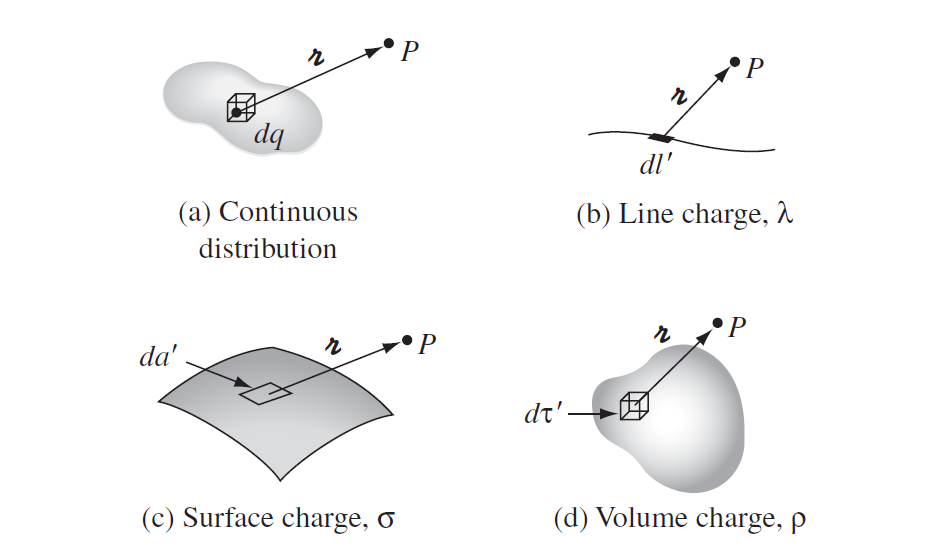
\includegraphics[height=6cm]{250-Revision/continuous-charge.png}
        \caption{Continuous charge distribution integration method (Fig 2.5 from Griffiths)}
        \label{fig:continuous-charge}
    \end{figure}
\end{itemize}

\subsection{Gauss's Law}
\subsubsection{Electric Field Lines}
    Suppose we have a point charge in $\mathbb{R}^3$ space and we are going to draw its electric field vectors. When we draw this vector field, we find that the vector arrows decay as being farther from the point charge.  Therefore, we need some other way to represent E field: electric field lines.
    \begin{figure}[ht]
        \centering
        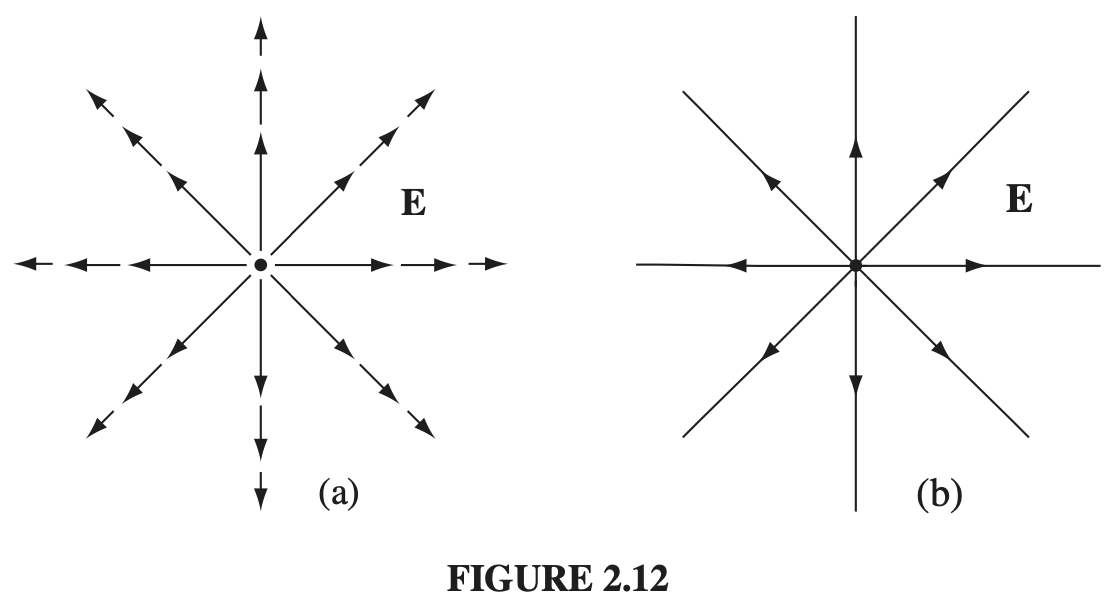
\includegraphics[height = 5cm]{250-Revision/Fig-2-12.png}
        \caption{Electric Field Vectors vs Electric Field Lines}
        \label{fig:field-lines}
    \end{figure}
    
    \begin{description}
        \item[Definition] Electric field lines are lines that connect the $\overrightarrow{E}$ vectors. In other words, $\overrightarrow{E}$ is tangential to field lines.
    \end{description}
    Some properties of field lines:
    \begin{itemize}
        \item Lines have to be continuous: one line appearing or disappearing, or two lines merging, would correspond to "expansions" or "contractions" of the $\overrightarrow{E}$ field.
        \item Lines cannot cross, unless there is a charge "emitting" or "absorbing" field lines. Only one vector value of the field at a given place.
        \item The density of lines tells about the magnitude of the field. (Note that it is meant to represent the slice of a 3D field.)
    \end{itemize}
    \begin{figure}
        \centering
        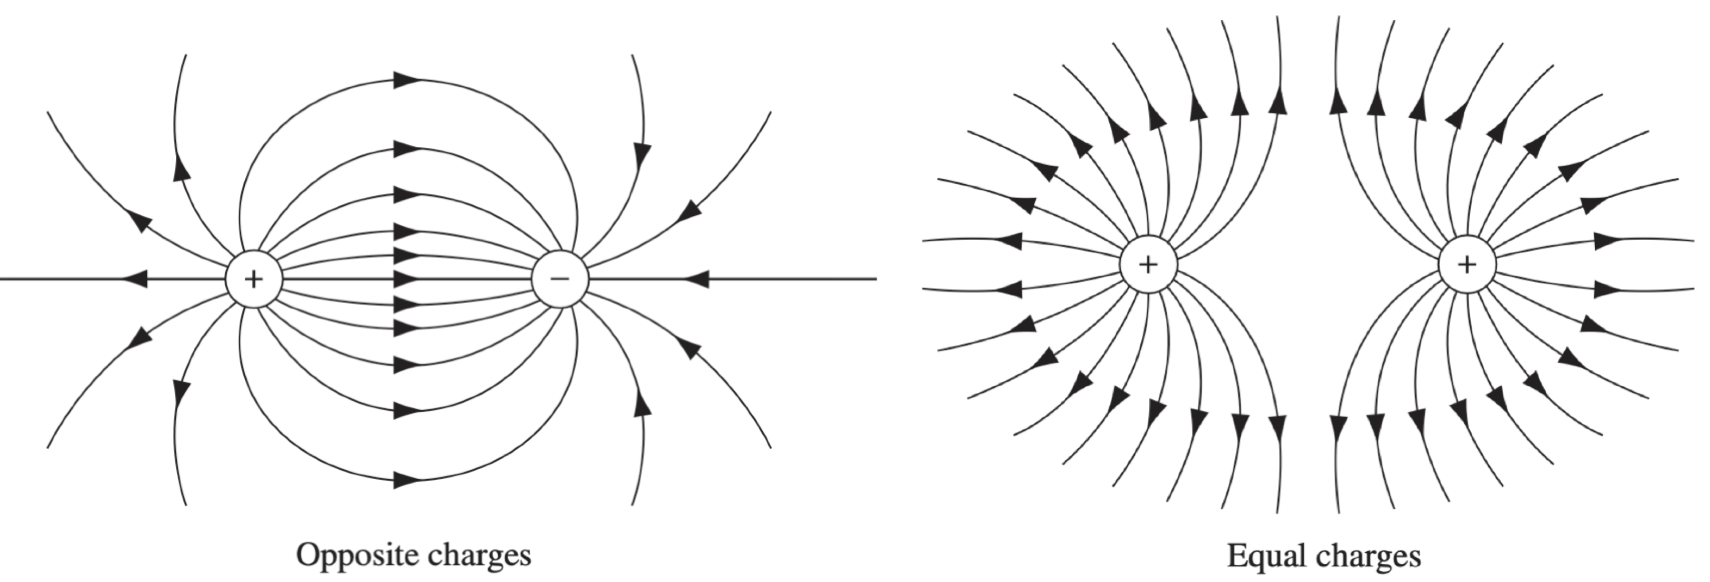
\includegraphics[width=12cm]{250-Revision/field-lines-eg.png}
        \caption{Field lines of two charges}
        \label{fig:field-line-eg}
    \end{figure}
    
\subsubsection{Gauss's Law}
    Consider a closed surface $\mathcal{S}$, then the flux of $\overrightarrow{E}$ on $\mathcal{S}$ will be:
    \begin{equation}
        \phi = \oiint_{\mathcal{S}}\overrightarrow{E}\cdot d\overrightarrow{a}
        \label{eq: e-flux}
    \end{equation}
    The electric field flux only depends on whether there exists net charge INSIDE the surface $\mathcal{S}$.
    \begin{itemize}
        \item If charge is inside the surface $\mathcal{S}$...
            \subitem The E field lines will cross the $\mathcal{S}$ outward and inward, unless net charge is zero. In this case, $\phi\neq 0$ (Figure 2.16(a))
        \item If charge is outside the surface $\mathcal{S}$...
            \subitem Then the E field lines will cross this closed surface twice, thus the net flux will be zero, i.e. $\phi=0$ (Figure 2.16(b))
        \begin{figure}[ht]
            \centering
            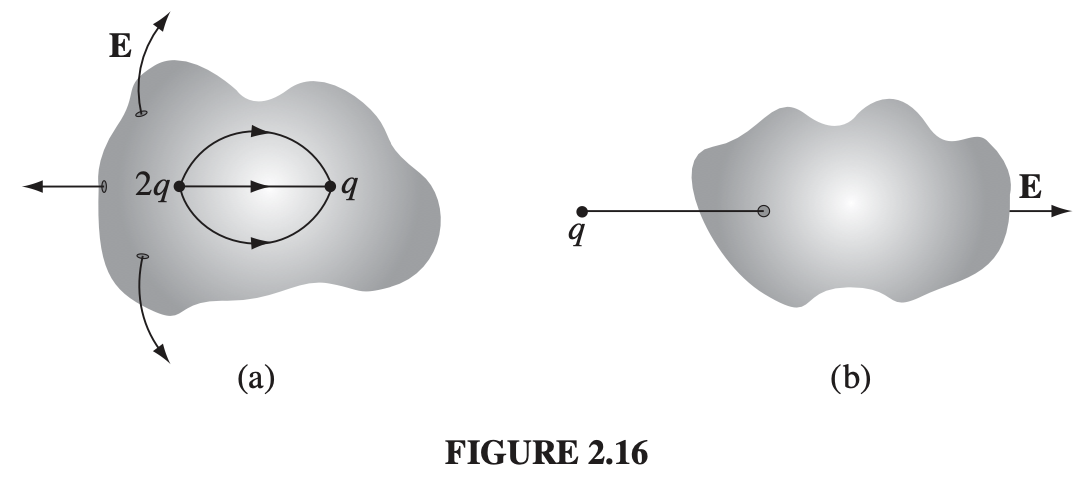
\includegraphics[width=10cm]{250-Revision/Fig-2-16.png}
            \caption{The E field flux depends on the position of charge.}
            \label{fig:2-16}
        \end{figure}
    \end{itemize}
    
    Now let's consider a sphere with radius $r$, which has a charge $q$ at its center. According to Coulomb's Law, the $\overrightarrow{E}$ is
    \[\overrightarrow{E} = \frac{1}{4\pi\varepsilon_0}\frac{q\hat{r}}{r^2}\]
    We want to know the flux of this E field, so we apply Equation \ref{eq: e-flux}, but before using this equation we need to evaluate the area element $\overrightarrow{a}$, since it is a sphere we use spherical coordinates:
    \[d\overrightarrow{a}=dl_\theta dl_\phi\hat{r}=r^2\sin\theta d\phi d\theta\hat{r}\]
    
    \[\oiint \overrightarrow{E}\cdot d\overrightarrow{a}=\frac{\cancel{r^2}q}{4\pi\varepsilon_0\cancel{r^2}}\underbrace{\int_{\phi=0}^{\phi=2\pi}d\phi\int_{\theta=0}^{\theta=\pi}\sin\theta d\theta}_{=4\pi}=\frac{q}{\varepsilon_0}\]
    
    (Note: Remember the value of the above double integral!)
    \newline
    \noindent Now, instead of a single charge, we have many charges, or even charges with continuous distributions. What will be the E field flux?\\
    \newline
    \noindent According to superposition principle of E field, the flux through a surface enclosing these charges will be the total flux of all E fields contributing to it:

        \begin{eqnarray*}
            \oiint \overrightarrow{E} \cdot d\overrightarrow{a} &=& \sum_{i=1}^{N}\left(\oiint \overrightarrow{E}_i \cdot d\overrightarrow{a}\right)  \\
            &=& \sum_{i=0}^{n}\frac{q_i}{\varepsilon_0}
        \end{eqnarray*}
        \begin{equation}
            \oiint \overrightarrow{E} \cdot d\overrightarrow{a}=\frac{Q_{\mathrm{enc}}}{\varepsilon_0}
            \label{eq: Gauss}
        \end{equation}
    And Equation \ref{eq: Gauss} is the \textbf{Gauss's Law} in math expression. In this equation, $Q_{\mathrm{enc}}$ is all charges enclosing in the surface; and to evaluate $Q_{\mathrm{enc}}$, refer to Equations 20, 21, 22.\\
    \newline
    \noindent Notice that Gauss's Law applies globally, but what if we want to make it be a local law? Gauss's Law also works, but we need to make some changes:
    \begin{itemize}
        \item According to divergence theorem, Gauss's integral can be written as:
        \[\oiint_\mathcal{S}\overrightarrow{E}\cdot d\overrightarrow{a}=\iiint_{\mathcal{V}}(\nabla\cdot \overrightarrow{E})d\tau\]
        
        \item In $\mathbb{R}^3$ space, the enclosed charge is:
        \[Q_{\mathrm{enc}}=\iiint \rho(\overrightarrow{r})d\tau\]
        (For point charge at origin, $\rho(\overrightarrow{r})=4\pi\delta^3(\overrightarrow{r})$)
        
        \item Use RHS of Gauss's Law (Eq. 24), and change the variables:
        \[\iiint_{\mathcal{V}}(\nabla\cdot \overrightarrow{E})d\tau=\frac{1}{\varepsilon_0}\iiint_{\mathcal{V}}\rho(\overrightarrow{r})d\tau\]
        
        \item Now we make $\mathcal{V}\to 0$, then the integral sign will automatically "take off":
        \[\iiint_{\mathcal{V}\to 0}(\nabla\cdot \overrightarrow{E})d\tau\approx (\nabla\cdot\overrightarrow{E})_{\overrightarrow{r}}\cancel{\mathcal{V}}=\left(\frac{\rho(\overrightarrow{r})}{\varepsilon_0}\right)_{\overrightarrow{r}}\cancel{\mathcal{V}}\]
        \begin{equation}
            \nabla \cdot \overrightarrow{E} = \frac{\rho(\overrightarrow{r})}{\varepsilon_0}
            \label{Eq: Maxwell-Gauss}
        \end{equation}
    \end{itemize}
    Equation \ref{Eq: Maxwell-Gauss} is also known as \textbf{Maxwell-Gauss Law} (\textit{First one in Maxwell Equations}), defining the value of divergence of E field. \textit{Alternative way to derive M-G Law, see Textbook p.71 and Lecture 7 notes.}

\subsubsection{Application of Gauss's Law}
    \begin{itemize}
        \item Spherical symmetry (\textit{Example 2.3, p.71}): we know total charge $q$ and radius of sphere $R$ (thus the density $\rho$), then what will be $\overrightarrow{E}$ outside sphere?
            \begin{itemize}
                \item First, check symmetry
                    \subitem $\overrightarrow{E}$ cannot depend on $\theta$ and $\phi$ values
                    \subitem $\overrightarrow{E}$ cannot depend on $\hat{\theta}$ and $\hat{\phi}$ direction. It only depends on $\hat{r}$
                    \subitem \(\overrightarrow{E}=E(r)\hat{r}\)
                \item Then, we integrate over the sphere, when $r>R$, then the surface at radius $r$ is called \textbf{Gaussian surface}:
                    \[d\overrightarrow{a}=r^2\sin\theta d\theta d\phi \hat{r}\]
                    \[\oiint \overrightarrow{E}\cdot d\overrightarrow{a}=r^2E(r)\int_{0}^{2\pi}d\phi\int_{0}^{2\pi}\sin\theta d\theta = 4\pi r^2E(r)\]
                    We also know that:
                    \[\phi=4\pi r^2E(r)=\frac{q}{\varepsilon_0}\]
                    Then:
                    \[\overrightarrow{E}=\frac{q}{4\pi r^2\varepsilon_0}\hat{r}\]
                \item This result shows that the E field outside sphere is the same as a point charge. (See Eq. 18)
            \end{itemize}
        
        \item Cylindrical symmetry (\textit{Example 2.4}): we know that the length of tube is infinite. We also know that the charge density is proportional to the distance from axis, i.e. $\rho =ks$. What is $\overrightarrow{E}$ inside this tube?
        \begin{figure}[ht]
            \centering
            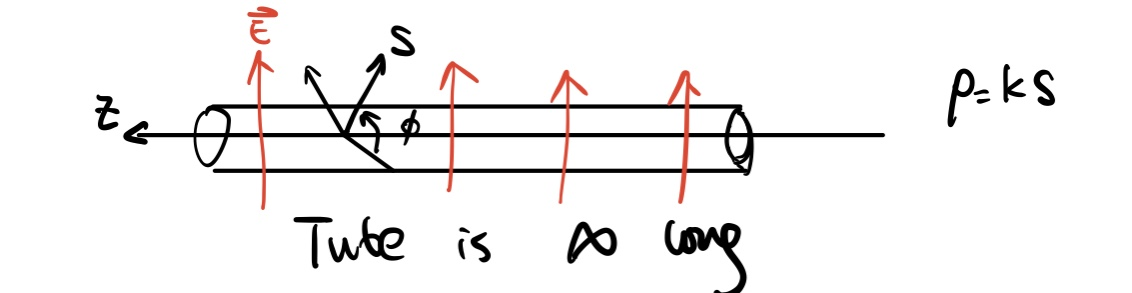
\includegraphics[width=7.5cm]{250-Revision/gauss-cylinder.png}
        \end{figure}
            \begin{itemize}
                \item Check symmetry:
                    \subitem Notice that, here we use cylindrical coordinates since it is a tube. In this example, $\overrightarrow{E}$ doesn't depend on $\phi$ and $z$ values, i.e. $\overrightarrow{E}(s)$
                    \subitem $\overrightarrow{E}$ along only on $\hat{s}$ direction, i.e. $\overrightarrow{E}(s)\hat{s}$
                \item Integrate the flux over cylinder of radius $s$ along $z$-axis with length $L$ (apply Gauss locally!), this will be our Gaussian surface.
                \begin{figure}[ht]
                    \centering
                    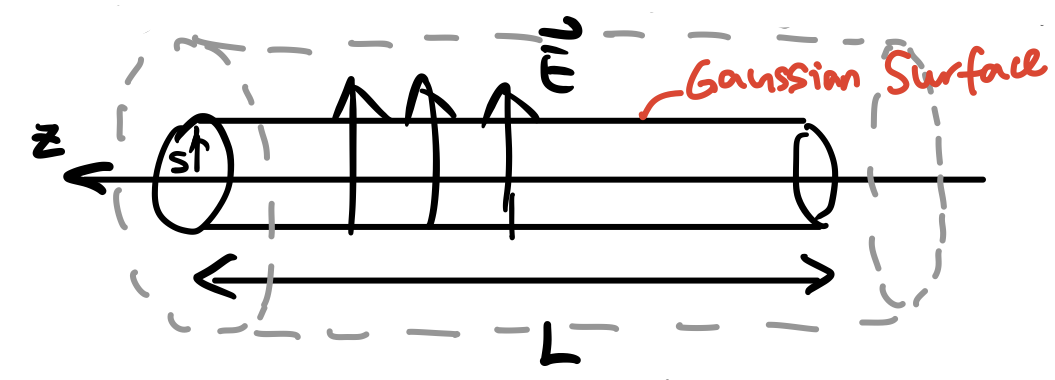
\includegraphics[width=7.5cm]{250-Revision/tube-gaussian-surface.png}
                \end{figure}
                    \subitem Notice that flux of sides don't contribute to total flux, since $\overrightarrow{E}\cdot \hat{z}=0$.
                    \subitem On the curved surface:
                    \[d\overrightarrow{a}=\hat{s}dzsd\phi\]
                    \[\oiint \overrightarrow{E}\cdot d\overrightarrow{a}=\int_{0}^{L}dz\int_{0}^{2\pi}E(s) sd\phi=2\pi sLE(s)\]
                \item Integrate $\rho(s)$ over cylinder to find $Q_{\mathrm{enc}}$:
                    \[Q_{\mathrm{enc}}=\iiint \rho(s)d\tau=\iiint \rho(s)dsdzsd\phi\]
                    \[=2\pi L\int_{0}^{s}k(s')^2ds'=\frac{2\pi kLs^3}{3}\]
                \item Apply Gauss Law:
                    \[\cancel{2\pi}\cancel{L}\cancel{s}E(s)=\frac{\cancel{2\pi} k\cancel{L}s^{\cancel{3}2}}{3\varepsilon_0}\]
                    \[\overrightarrow{E}(s)=\frac{ks^2}{3\varepsilon_0}\hat{s}\]
            \end{itemize}
            
        \item Cartesian symmetry (\textit{Ex. 2.5})
            \begin{figure}[ht]
                \centering
                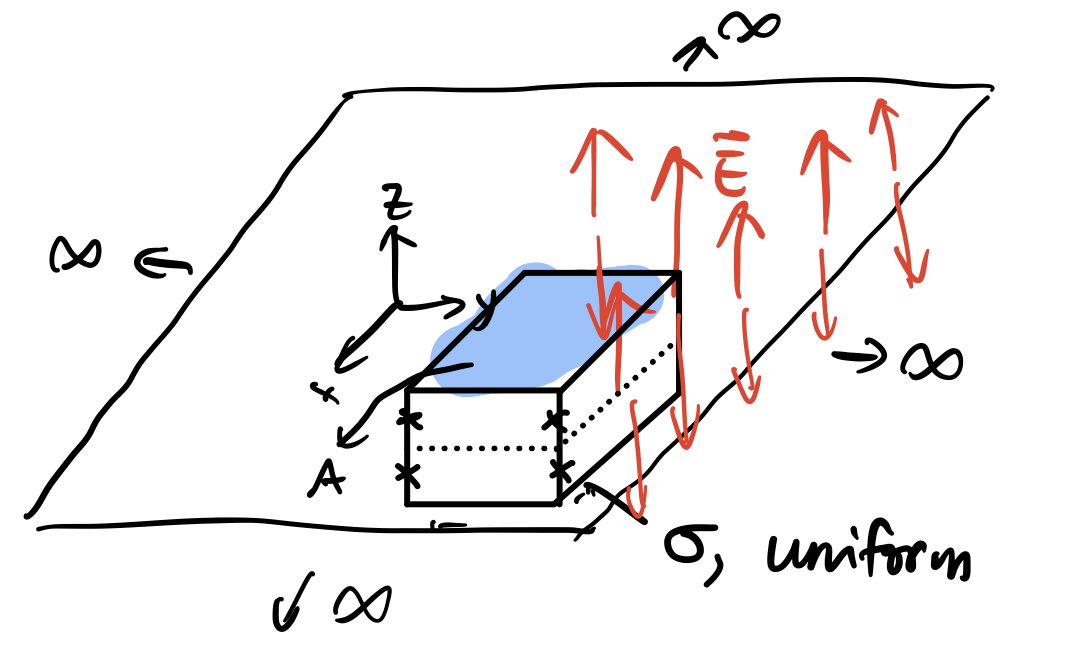
\includegraphics[width = 8cm]{250-Revision/gauss-cartesian.png}
            \end{figure}
            An infinite plane carries a uniform surface charge $\sigma$, find the E field.
            \begin{itemize}
                \item Check symmetry
                    \subitem $\overrightarrow{E}$ does not depend on $x, y$, and has to be along $\hat{z}$ direction. i.e. $\overrightarrow{E}=E(z)\hat{z}$
                \item Integrate flux:
                    \subitem Draw a pillbox extending equal distances above and below the plane, this will be our Gaussian surface.
                    \subitem Sides won't contribute: $\overrightarrow{E}\cdot \hat{x}=\overrightarrow{E}\cdot\hat{y}=0$
                    \[d\overrightarrow{a}_{\mathrm{top}}=dxdy\hat{z}\]
                    \[d\overrightarrow{a}_{\mathrm{bottom}}=-dxdy\hat{z}\]
                    \subitem On top and bottom surfaces:
                    \[\iint_{\mathrm{top+bottom}}\overrightarrow{E}\cdot d\overrightarrow{a}=E(z)A\] 
                    \[\oiint \overrightarrow{E}\cdot \overrightarrow{a}=\iint_{\mathrm{top}}\overrightarrow{E}\cdot \overrightarrow{a}+\iint_{\mathrm{bottom}}\overrightarrow{E}\cdot \overrightarrow{a}=2AE(z)\]
                \item
                \[Q_{\mathrm{enc}}=\sigma A\]
                \item Apply Gauss's Law:
                \[2AE(z)=\frac{\sigma A}{\varepsilon_0}\implies E(z)=\frac{\sigma }{2\varepsilon_0}\]
                \[\overrightarrow{E}_{\mathrm{abv}}=\frac{\sigma }{2\varepsilon_0}\hat{z}\]
                \[\overrightarrow{E}_{\mathrm{blw}}=-\frac{\sigma }{2\varepsilon_0}\hat{z}\]
            \end{itemize}
    \end{itemize}
    To summarize, there are three symmetries that can work:
    \begin{enumerate}
        \item \textbf{Spherical symmetry}: Gaussian surface is a concentric sphere.
        \item \textbf{Cylindrical symmetry}: Gaussian surface is a coaxial cylinder.
        \item \textbf{Cartesian symmetry}: Gaussian surface/pillbox is a pillbox that the surface can pass through it.
    \end{enumerate}
    \begin{figure}[ht]
        \centering
        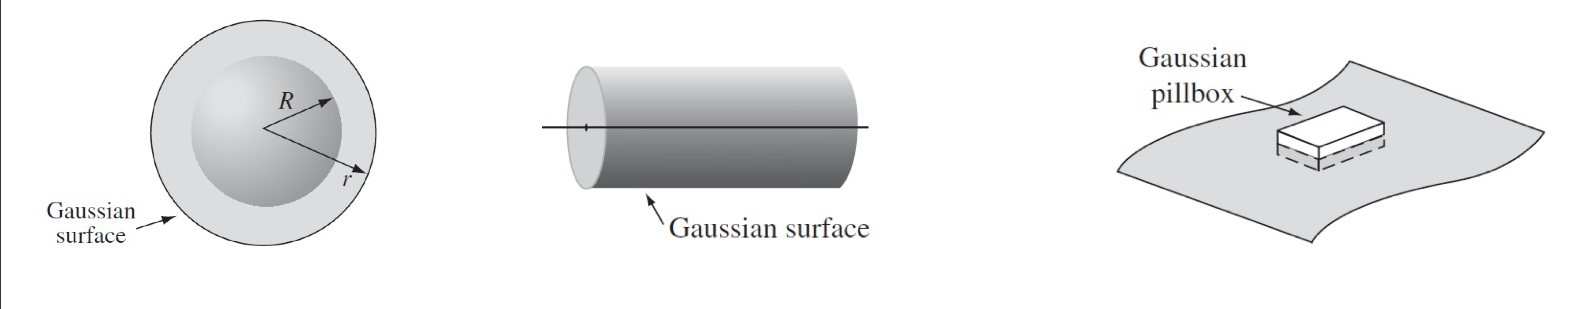
\includegraphics[width=15cm]{250-Revision/gaussian-surfaces.png}
        \caption{Selection of Gaussian surfaces}
        \label{fig:gaussian-surfaces}
    \end{figure}
    \textit{Exercise: Eg. 2.6, p.75}
    
\subsubsection{Curl of E field}
    \[\nabla \times \overrightarrow{E}=0\]
    \textit{See textbook p.78-79, and try completing problem 2.19}\\
    Let's consider a single point charge, where the electric field is:
    \[\overrightarrow{E}=\frac{q}{4\pi\varepsilon_0r^2}\hat{r}\]
    We want to evaluate the curl of E field, which is somewhat hard to start with. However, thanks to Stokes' theorem, we can evaluate the closed line integral first.
    \[\int_{\overrightarrow{a}}^{\overrightarrow{b}}\overrightarrow{E}\cdot d\overrightarrow{l}=\int_{||\mathbf{a}||}^{||\mathbf{b}||}\frac{q}{4\pi\varepsilon_0 r^2}dr=\frac{q}{4\pi\varepsilon_0}\left(\frac{1}{a}-\frac{1}{b}\right)\]
    If the path closed, i.e. $a=b$, by using Stokes' Theorem
    \[\oint_{\mathcal{P}}\overrightarrow{E}\cdot d\overrightarrow{l}=0\iff \iint_{\mathcal{S}}(\nabla\times \overrightarrow{E})\cdot d\overrightarrow{a}=0\]
    We shrink the path and surface $\mathcal{P}, \mathcal{S}$ to zero, then:
    \[\mathcal{P},\mathcal{S}\to 0\implies (\nabla \times \overrightarrow{E})\cdot d\overrightarrow{a}=0\]
    $\forall d\overrightarrow{a}$,  we always have the following equation:
    \begin{equation}
        \nabla \times \overrightarrow{E} = \overrightarrow{0}
        \label{eq: Maxwell-Faraday equation}
    \end{equation}
    And this is called \textbf{Maxwell-Faraday Equation}, which is true for $\partial \overrightarrow{B}/\partial t=0$.
\subsection{Electric Potential}
\subsubsection{Electric Potential}
    In last section (2.2.4), we have generally shown that the curl of E field is always zero. This implies that:
    \[\nabla\times \overrightarrow{E}=\overrightarrow{0}\iff \overrightarrow{E}=-\nabla V\]
    Let $V(\overrightarrow{r})=-\int_{\overrightarrow{r_0}}^{\overrightarrow{r}}\overrightarrow{E}\cdot d\overrightarrow{l}$, this is called \textbf{Electric potential}. Then:
    \[V(\overrightarrow{b})-V(\overrightarrow{a})=-\int_{\overrightarrow{r_0}}^{\overrightarrow{b}}\overrightarrow{E}\cdot d\overrightarrow{l}+\int_{\overrightarrow{r_0}}^{\overrightarrow{a}}\overrightarrow{E}\cdot d\overrightarrow{l}=-\int_{\overrightarrow{a}}^{\overrightarrow{b}}\overrightarrow{E}\cdot d \overrightarrow{l}\]
    By fundamental theorem of gradient:
    \[V(\overrightarrow{b})-V(\overrightarrow{a})=\int_{\overrightarrow{a}}^{\overrightarrow{b}}(\nabla V)\cdot d\overrightarrow{l}\]
    \[\implies \int_{\overrightarrow{a}}^{\overrightarrow{b}}(\nabla V)\cdot d\overrightarrow{l}=-\int_{\overrightarrow{a}}^{\overrightarrow{b}}\overrightarrow{E}\cdot d \overrightarrow{l}\]
    We make $\overrightarrow{b}-\overrightarrow{a}\to \overrightarrow{0}$, then:
        \begin{equation}
            \overrightarrow{E}=-\nabla V
            \label{eq: E-V equation}
        \end{equation}
    Where $V$ is called electric potential.\\
    \newline
    \noindent Back to our definition of electric potential, we wonder how to choose $\overrightarrow{r_0}$...
    \begin{equation}
        V(\overrightarrow{r})=-\int_{\overrightarrow{r_0}}^{\overrightarrow{r}}\overrightarrow{E}\cdot d\overrightarrow{l}
        \label{eq:potential}
    \end{equation}
    \begin{itemize}
        \item For practical purpose I: $\overrightarrow{r_0}$ in fact doesn't matter because we usually evaluate the potential differences instead of potential at one location, or we evaluate the gradient of potential ($\nabla V$).
        From Prof Grizouard's Lecture Notes, changing $\overrightarrow{r_0}$ adds the same constant to all values of $V$, and it disappears when doing these operations.
        
        \item Practical purpose II: Choose what it most convenient.
        
        By default:
        \begin{itemize}
            \item For spherical problems:
            \[\lim_{r\to\infty}V(r)=0\implies V=-\int_{\infty}^{\overrightarrow{r}}\overrightarrow{E}\cdot d\overrightarrow{l}\]
                \textit{Exercise: Ex 2.7}
            \item For cylindrical problems: choose some points off the axis (see tutorial)
            \item For infinite plates: choose some $\overrightarrow{r_0}$ on the plate.
        \end{itemize}
    
    \end{itemize}

\subsubsection{Superposition Principle of Electric Potential and Continuous Distribution}
    The superposition of electric potential is very similar to that in electric field.
    \begin{equation}
        V_T=-\int_{\overrightarrow{r_0}}^{\overrightarrow{r}}\overrightarrow{E}\cdot d\overrightarrow{l}=-\int_{\overrightarrow{r_0}}^{\overrightarrow{r}}\sum_{i=1}^{N}\overrightarrow{E}_i\cdot \overrightarrow{l}=-\sum_{i=1}^{N}\int_{\overrightarrow{r_0}}^{\overrightarrow{r}}\overrightarrow{E}_i\cdot \overrightarrow{l}=\sum_{i=1}^{N}V_i
        \label{eq: V-superposition}
    \end{equation}
    For continuous distributions, we use the same idea:
    \begin{itemize}
        \item 3D:
        \begin{equation}
            V=\frac{1}{4\pi\varepsilon_0}\iiint \frac{\rho(\overrightarrow{r'})}{\rc}d\tau
        \end{equation}
        \item 2D:
        \begin{equation}
            V=\frac{1}{4\pi\varepsilon_0}\iint \frac{\sigma(\overrightarrow{r'})}{\rc}da
        \end{equation}
        \item 1D:
        \begin{equation}
            V=\frac{1}{4\pi\varepsilon_0}\int \frac{\lambda(\overrightarrow{r'})}{\rc}dl
        \end{equation}
    \end{itemize}
    \textit{Exercise: Ex. 2.8, Pb. 2.25b, see Lecture 9 notes.}

\subsection{Electrostatic Potential Energy}
\subsubsection{EPE-Introduction}
    \textbf{REMEMBER: Electrostatic PE $\neq$ Electrostatics Potential!}\\
    \noindent Now we want to move a test charge $Q$ from $\overrightarrow{a}$ to $\overrightarrow{b}$. How much work is done during this movement?
    \begin{figure}[ht]
        \centering
        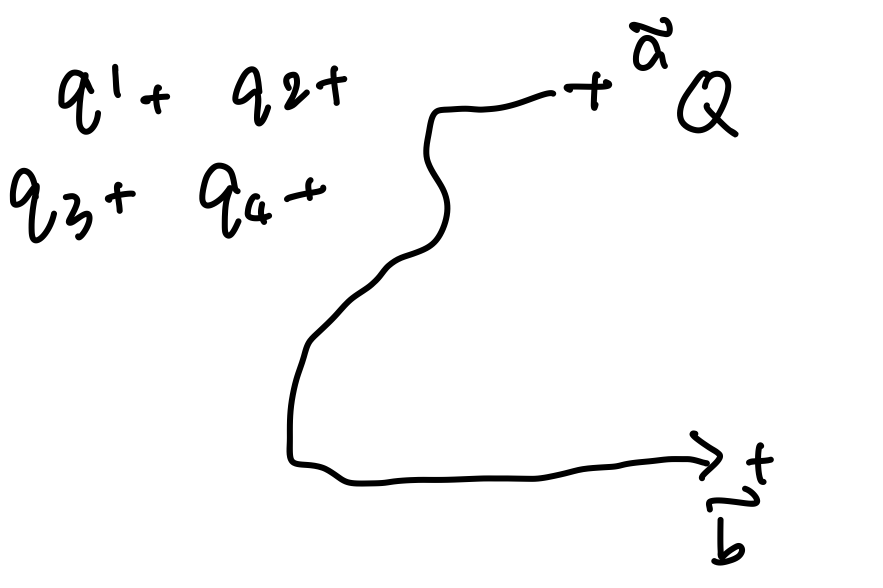
\includegraphics[width=5cm]{250-Revision/pe-moving-charge.png}
    \end{figure}
    
    \noindent First, according to Coulomb's Law, the Coulomb force is:
    \[\overrightarrow{F}=Q\overrightarrow{E}\]
    
    \noindent From PHY254 knowledge, the work done against the electrostatic force by the mover is:
    \begin{eqnarray*}
    W &=& -\int_{\overrightarrow{a}}^{\overrightarrow{b}}\overrightarrow{F}\cdot d\overrightarrow{l}\\
    &=& -\int_{\overrightarrow{a}}^{\overrightarrow{b}}(Q\overrightarrow{E})\cdot d\overrightarrow{l}\\
    &=& +Q\int_{\overrightarrow{a}}^{\overrightarrow{b}}(\nabla V)\cdot d\overrightarrow{l}\\
    &=& Q(V(\overrightarrow{b})-V(\overrightarrow{a}))
    \end{eqnarray*}
    \begin{itemize}
        \item Unit of work is Joule (J)
        \item It would be the only energy gained/lost by Q if motion was infinitely slow and no other force was present.
        \item Notice that, \(V(\overrightarrow{b})-V(\overrightarrow{a})=W/Q\), or \textbf{the potential difference is the work required to move charge from} $\overrightarrow{a}$ \textbf{to} $\overrightarrow{b}$ \textbf{per} \textbf{unit charge}.
        \item If we bring the charge from infinitely far away to $\overrightarrow{r}$, then...
        \[W=Q(V(\overrightarrow{r})-V_\infty)=QV(\overrightarrow{r})\]
        \item From PHY254: $W=+U$, where $U$ is the potential energy. Notice the plus sign before $U$, and note that not all authors use the same sign conventions.
            \subitem Therefore, $V$ is the potential energy per unit charge, i.e. in 1st year physics course, $V=PE/q=kQ/r,\ PE=kqQ/r$.
    \end{itemize}

\subsubsection{EPE for discrete charges collection}
    \begin{itemize}
        \item Introduce $q_1$, then
        \[V_1=\frac{q_1}{4\pi\varepsilon_0r'_1}\]
        \item Bring $q_2$:
        \[W_2=q_2V_1=\frac{1}{4\pi\varepsilon_0}\frac{q_1q_2}{\rc_{1,2}}\]
        where \(\rc_{1,2}=||\overrightarrow{r_2'}-\overrightarrow{r_1'}||\)
        \item Bring $q_3$:
        \[W_3=q_3V_{1,2}=\frac{1}{4\pi\varepsilon_0}q_3\left(\frac{q_1}{\rc_{1,3}}+\frac{q_2}{\rc_{2,3}}\right)\]
        where $V_{1,2}$ is potential due to $q_1$ and $q_2$.
        And the total work up to here will be...
        \[W_T=\frac{1}{4\pi\varepsilon_0}\left(\frac{q_1q_2}{\rc_{1,2}}+\frac{q_2q_3}{\rc_{2,3}}+\frac{q_1q_3}{\rc_{1,3}}\right)\]
        \item Bring $q_4$:
        \[W_4=\frac{1}{4\pi\varepsilon_0}q_4\left(\frac{q_1}{\rc_{1,4}}+\frac{q_2}{\rc_{2,4}}+\frac{q_3}{\rc_{3,4}}\right)\]
        \begin{eqnarray*}
            W_T &=& \frac{1}{4\pi\varepsilon_0}\left(\frac{q_1q_2}{\rc_{1,2}}+\frac{q_2q_3}{\rc_{2,3}}+\frac{q_1q_3}{\rc_{1,3}}+\frac{q_1q_4}{\rc_{1,4}}+\frac{q_2q_4}{\rc_{2,4}}+\frac{q_3q_4}{\rc_{3,4}}\right)\\
            &=& \frac{1}{4\pi\varepsilon_0}\sum_{i=1}^{4}\sum_{j>1}^{4}\frac{q_iq_j}{\rc_{i,j}}
        \end{eqnarray*}
        
        \item $N$ charges:
        \begin{equation}
            W=\frac{1}{4\pi\varepsilon_0}\sum_{i=1}^{N}\sum_{j> i}^{N}\frac{q_iq_j}{\rc_{i,j}}
        \end{equation}
        If we directly apply $N$ for the double summation with index $j\neq i$, we will double count $q_iq_j$ and $q_jq_i$, so we need to divide by 2:
        \begin{equation}
            W=\frac{1}{8\pi\varepsilon_0}\sum_{i=1}^{N}\sum_{j\neq i}^{N}\frac{q_iq_j}{\rc_{i,j}}
        \end{equation}
        Alternatively:
        \begin{equation}
            W=\frac{1}{8\pi\varepsilon_0}\sum_{i=1}^{N}q_i\sum_{j\neq i}^{N}\frac{q_j}{\rc_{i,j}}=\frac{1}{2}\sum_{i=1}^{N}q_iV_i(\overrightarrow{r_i'})
        \end{equation}
        where $V_i(\overrightarrow{r_i'})$ is potential due to all other charges, and 
        \[V_i(\overrightarrow{r_i'})=\frac{1}{4\pi\epsilon_0}\sum_{j\neq i}\frac{q_j}{\rc_{i,j}}\]
    \end{itemize}
    \textit{Exercise: Pb. 2.31(a)}
    
\subsubsection{EPE for continuous distribution of charges}
    Just replace $\sum q_i$ with $\iiint \rho d\tau$:
    \begin{equation}
        W=\frac{1}{2}\iiint_{\textrm{q distrib}} \rho(\overrightarrow{r'})V(\overrightarrow{r'})d\tau
    \end{equation}
    Some nice formula...
    \[\nabla \cdot(f\overrightarrow{A})=f(\nabla\cdot \overrightarrow{A})+\overrightarrow{A}\cdot (\nabla f),\ \rho =\varepsilon_0(\nabla \cdot \overrightarrow{E})\]
    This implies
    \begin{eqnarray*}
        \rho V &=& \varepsilon_0 (\nabla \cdot \overrightarrow{E})V\\
        &=& \varepsilon_0[\nabla \cdot(V\overrightarrow{E})-\overrightarrow{E}\cdot\underbrace{\nabla V}_{-\overrightarrow{E}}]\\
        &=& \varepsilon_0[\nabla\cdot (V\overrightarrow{E})+||\overrightarrow{E}||^2]\\
        (\nabla\cdot(V\overrightarrow{E})&=& V(\nabla \cdot \overrightarrow{E})+\overrightarrow{E}\cdot(\nabla V))
    \end{eqnarray*}
    \[\implies W= \frac{\varepsilon_0}{2}\iiint[\nabla\cdot (V\overrightarrow{E})+||\overrightarrow{E}||^2]d\tau\]
    Use divergence theorem:
    \[\iiint \nabla \cdot (V\overrightarrow{E})d\tau=\oiint V\overrightarrow{E}\cdot d\overrightarrow{a}\]
    Assume $\rho(r)$ is compact, i.e. pushing volume boundaries to infinity: from far away, all localize charge distributions will look like point charges. Then:
    \[V=\frac{q}{4\pi\varepsilon_0 r},\ \overrightarrow{E}=\frac{q}{4\pi\varepsilon_0 r^2}\hat{r}\]
    where $q=\iiint \rho d\tau$ with whole distribution.\\
    \noindent Then:
    \[\oiint V\overrightarrow{E}\cdot d\overrightarrow{a}=4\pi r^2\cdot \frac{q^2}{(4\pi \varepsilon_0)^2r^3}=\frac{q^2}{4\pi\varepsilon_0^2 r}\]
    While
    \[\lim_{r\to\infty}\frac{q^2}{4\pi\varepsilon_0^2 r}=0\]
    Finally, integrating over whole $\mathbb{R}^3$ space:
    \[W=\frac{\varepsilon_0}{2}\iiint_{\mathbb{R}^3}||\overrightarrow{E}||^2d\tau\]
\subsubsection{EPE don't superpose}
    For two charges $q_1, q_2$:
        \[\overrightarrow{E} = \overrightarrow{E_1}+\overrightarrow{E_2}\]
        \begin{eqnarray*}
        W_T &=& \frac{\varepsilon_0}{2}\iiint ||\overrightarrow{E_1}+\overrightarrow{E_2}||^2d\tau\\
        &=& \frac{\varepsilon_0}{2}\iiint(E_1^2+E_2^2+2\overrightarrow{E_1}\cdot \overrightarrow{E_2})d\tau\\
        &=& W_1+W_2+\frac{\varepsilon_0}{2}\iiint (\overrightarrow{E_1}\cdot\overrightarrow{E_2})d\tau
        \end{eqnarray*}
\subsection{Conductors and Capacitance}
\subsubsection{Conductors}
    \begin{description}
        \item[Definition] An ideal conductor is that charges move as in free space, and there is no friction, i.e. $\sum \overrightarrow{F}=m\overrightarrow{a}=q\overrightarrow{E}$.
    \end{description}
    Some consequences of being an ideal conductor:
    \begin{enumerate}
        \item $\overrightarrow{E}=\overrightarrow{0}$ inside (in electrostatic limit).
        \begin{figure}[ht]
            \centering
            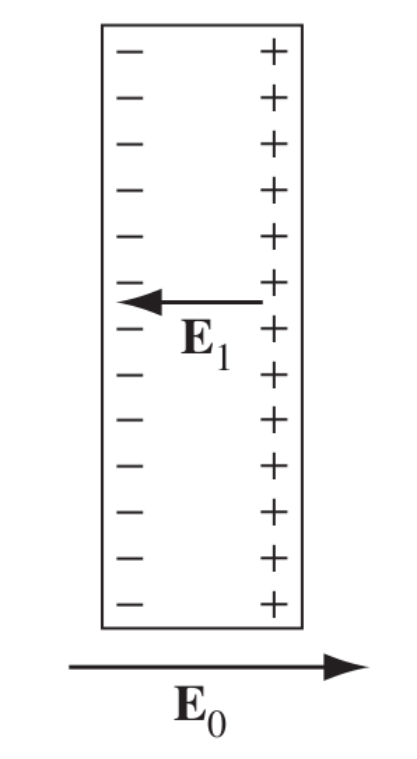
\includegraphics[height=5cm]{250-Revision/fig-2.42.png}
            \caption{Fig 2.42 from Griffiths. In this figure, \textbf{E0} is the external electric field, and \textbf{E1} is induced electric field. Therefore total electric field = \textbf{E1} + \textbf{E0} = \textbf{0}}
            \label{fig:2.42}
        \end{figure}
        \item Inside conductor:
            \subitem \(\rho=\varepsilon_0\nabla \cdot \overrightarrow{E}\)
            \subitem \(\overrightarrow{E}=0\implies\rho=0\)
            \subitem This is derived from Maxwell-Gauss Law.
        
        \item \(\overrightarrow{E}(\mathrm{inside})=-\nabla V(\mathrm{inside})=\overrightarrow{0}\implies V=\mathrm{constant}\)\\
        This means that any net charges (metal: electrons, electrolyte: ions, plasma: electrons and positive nuclei) are on surface, and inside these, there might exist some charges but the net charge is always zero. Therefore a conductor is a \textbf{equipotential body}.
        
        \item \(\overrightarrow{E}\perp\) surface near the surface
        \begin{figure}[ht]
            \centering
            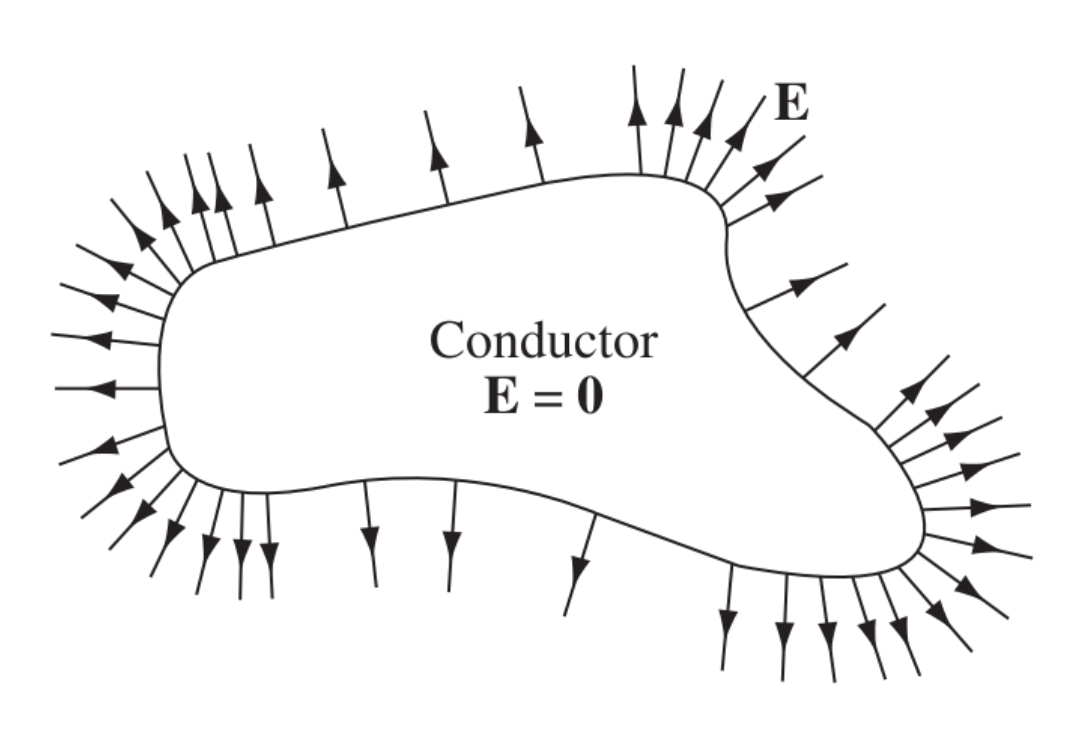
\includegraphics[width=7cm]{250-Revision/fig-2.43.png}
            \label{fig:2.43}
        \end{figure}
        
        Let's first consider a Gaussian pillbox for very small thickness:
        \begin{figure}[ht]
            \centering
            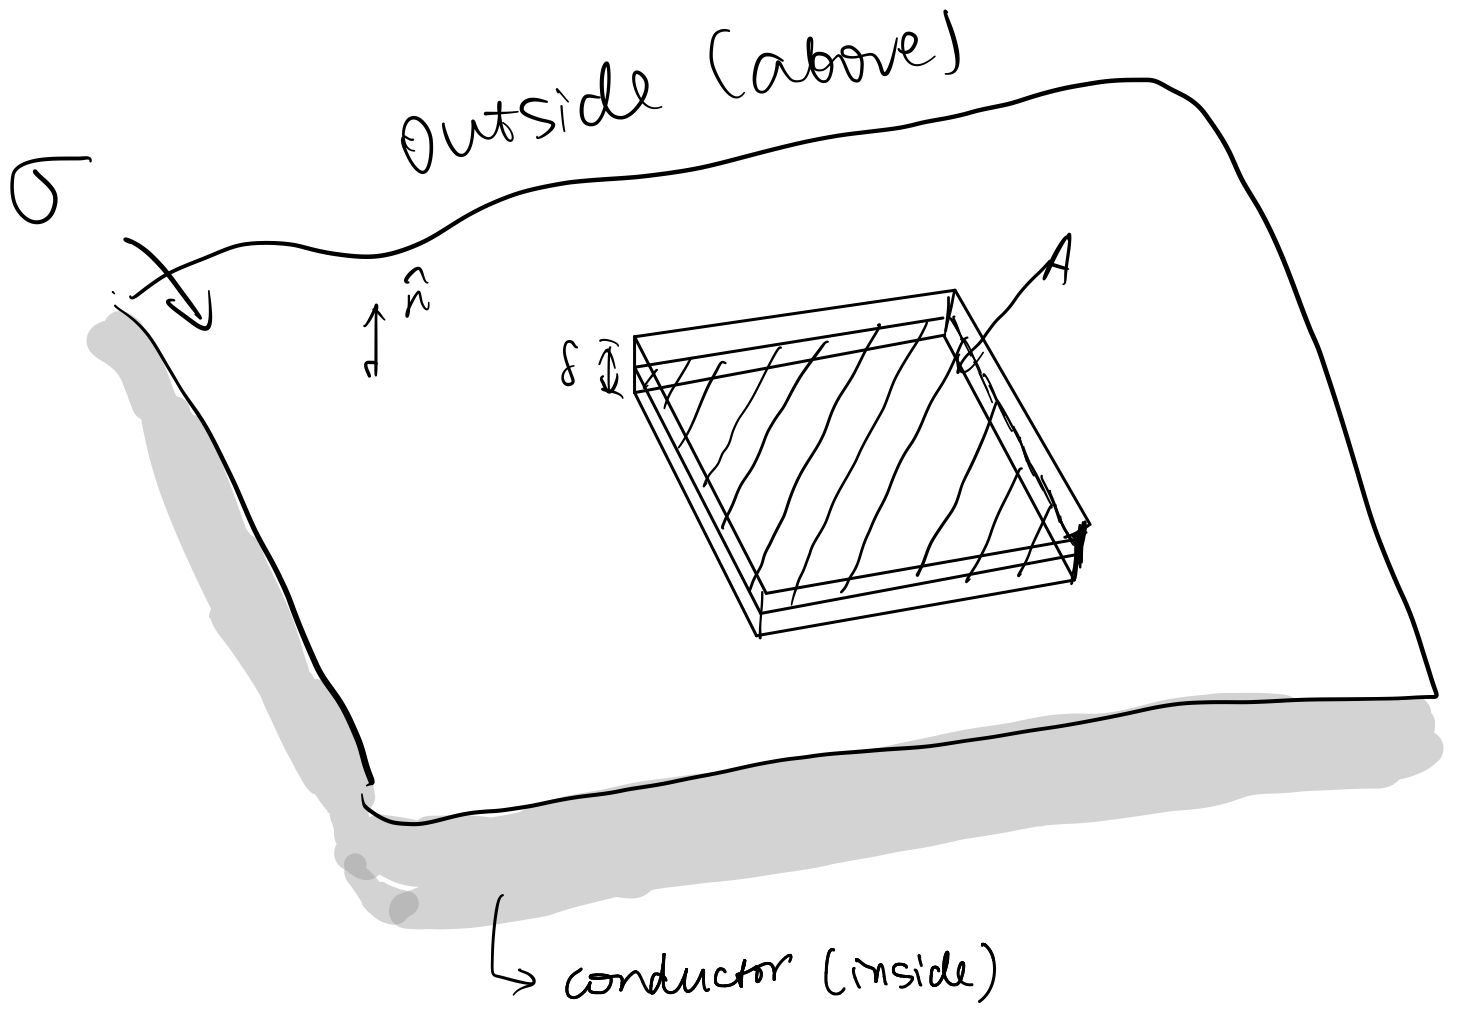
\includegraphics[width=7cm]{250-Revision/gaussian-pillbox-conductor.png}
        \end{figure}
        
        According to Gauss's Law, for a tiny pillbox around surface:
        \[\oiint \overrightarrow{E}\cdot d\overrightarrow{a}=\frac{\sigma A}{\varepsilon_0}\]
        Now let's vanish the thickness to zero, i.e. $\delta\to 0$, therefore the sides won't contribute to flux.
        Inside the conductor, total E field is zero, then for some small area $A$:
        \[\oiint \overrightarrow{E}_{T}\cdot d\overrightarrow{a}=E^{\perp}_{\mathrm{out}}A=\frac{\sigma A}{\varepsilon_0}\]
        \[E^{\perp}_{\mathrm{out}}=\frac{\sigma}{\varepsilon_0}\]
        
        How about the E field parallel to surface, i.e. $\overrightarrow{E}_\parallel$? Use Stokes' Theorem.
        \begin{figure}[ht]
            \centering
            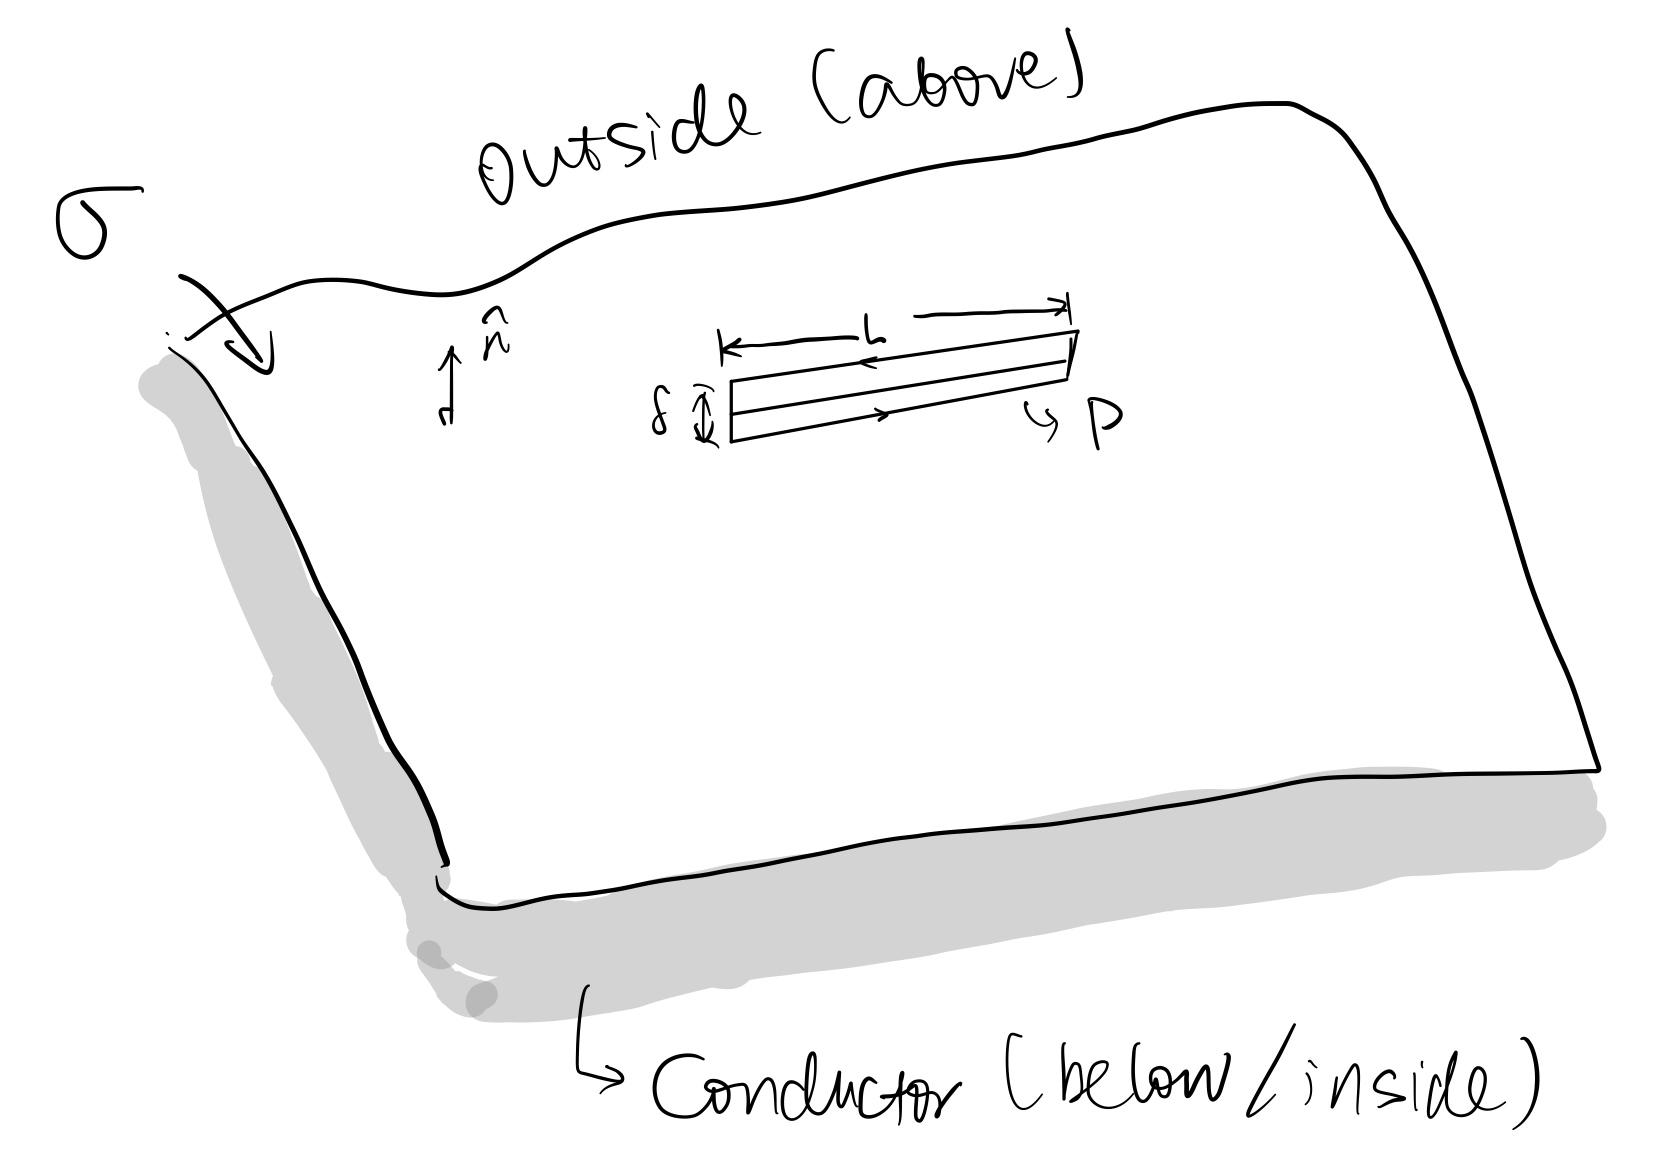
\includegraphics[width=7cm]{250-Revision/gaussian-pillbox-conductor-2.png}
        \end{figure}
        
        $E_{\parallel}$ circulate $\overrightarrow{E}$ over $\mathcal{P}$:
        \[\nabla\times \overrightarrow{E}=\overrightarrow{0}\iff \oint_{\mathcal{P}}\overrightarrow{E}\cdot d\overrightarrow{l}=\overrightarrow{0}\]
        \[\implies \cancel{E^{\parallel}_{\mathrm{below}}} - E^{\parallel}_{\mathrm{above}}L=0\]
        \[E_{\parallel}=0\]
        
        Finally:
        \[\overrightarrow{E}_{\mathrm{out}}=\overrightarrow{E}_{\perp}=\frac{\sigma}{\varepsilon_0}\hat{n}\]
        (\textit{For more, see Sect 2.3.5 on p.88-90})
        
        \item Conductor is an equipotential body. (Derived from item 3)
    \end{enumerate}
    \textit{Exercise: Pb. 2.38}

\subsubsection{Capacitors and Capacitance}
    First, let's focus on force on a conductor and its electrostatic pressure. Consider a surface with charge density $\sigma$.
    \begin{figure}[ht]
        \centering
        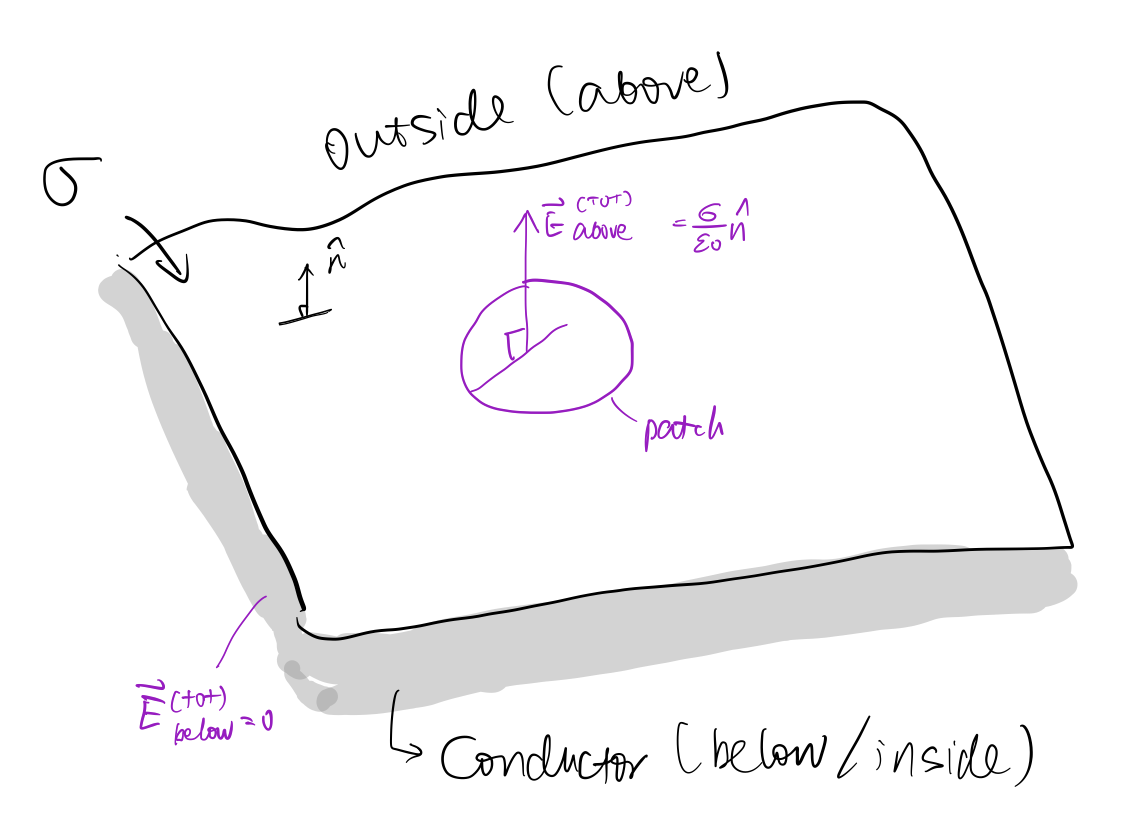
\includegraphics[width=7cm]{250-Revision/L12-pressure.png}
    \end{figure}
    
    \noindent Then the electric force on a patch per unit area:
    \[\overrightarrow{F}=\sigma \overrightarrow{E}_{\mathrm{other}}\]
    where $\overrightarrow{E}_{\mathrm{other}}$ is the field induced by \textit{anything but} the patch itself.\\
    \newline
    \noindent We also know that:
    \[\overrightarrow{E}_{T,\mathrm{blw}}=\overrightarrow{0},\ \overrightarrow{E}_{T,\mathrm{abv}}=\frac{\sigma }{\varepsilon_0}\hat{n}\]
    Besides:
    \[\overrightarrow{E}_{\mathrm{patch,abv}}=\frac{\sigma}{2\varepsilon_0}\hat{n},\ \overrightarrow{E}_{\mathrm{patch,blw}}=-\frac{\sigma}{2\varepsilon_0}\hat{n}\]
    (\textit{See Lec 8 for more about 2 in the denominator, by using Cartesian symmetry})\\
    
    \noindent Then \(\overrightarrow{E}_T=\overrightarrow{E}_{\mathrm{patch}}+\overrightarrow{E}_{\mathrm{other}}\), but \(\overrightarrow{E}_{\mathrm{other,abv}}=\overrightarrow{E}_{\mathrm{other,blw}}\) since it is not created by the patch. Therefore:
    \[\overrightarrow{E}_{T,\mathrm{abv}}=\frac{\sigma}{2\varepsilon_0}\hat{n}+\overrightarrow{E}_{\mathrm{other}}\]
    \[\overrightarrow{E}_{T,\mathrm{blw}}=-\frac{\sigma}{2\varepsilon_0}\hat{n}+\overrightarrow{E}_{\mathrm{other}}\]
    \[\implies \overrightarrow{E}_{\mathrm{other}}=\frac{1}{2}(\overrightarrow{E}_{T,\mathrm{abv}}+\overrightarrow{E}_{T,\mathrm{blw}})=\frac{\sigma}{2\varepsilon_0}\hat{n}\]
    (\textit{average value of above and below})
    
    \[\implies \overrightarrow{F}=\sigma\overrightarrow{E}_{\mathrm{other}}=\frac{\sigma^2}{2\varepsilon_0}\hat{n}=\frac{\varepsilon_0||\overrightarrow{E}_{T,\mathrm{abv}}||^2\hat{n}}{2}\]
    And its magnitude is called \textbf{electrostatic pressure}:
    \begin{equation}
        P=\frac{\varepsilon_0E^2}{2}
    \end{equation}
    \textit{Exercise: Pb. 2.41, p.104}\\
    \newline
    
    \noindent \textbf{CAPACITORS}
    \begin{description}
        \item[Definition] A capacitor consists of two conductors with opposite total charges, separated by insulator.
    \end{description}
    Recall that:
    \[V_{(+)}-V_{(-)}=-\int_{(-)}^{(+)}\overrightarrow{E}\cdot d\overrightarrow{l}=V\]
    And now we accept the fact that:
    \[V\propto Q\implies Q=CV\]
    Then, the proportionality constant $C$ of the above equation is called \textbf{capacitance}:
    \begin{equation}
        C=\frac{Q}{V}
        \label{eq:capacitance}
    \end{equation}
    
    \textit{Exercise: Ex. 2.11/12, p.106}\\
    \newline
    
    \noindent Also recall that, $W=Q(V(\overrightarrow{b})-V(\overrightarrow{a}))$, then we have the following ODE:
    \[dw=vdq=\frac{qdq}{C}\]
    \[W=\int_0^Q\frac{qdq}{C}=\frac{1}{2}\frac{Q^2}{C}\]
    \begin{equation}
        W=\frac{1}{2}CV^2
        \label{eq: Capacitor-energy}
    \end{equation}
    which is the energy stored in the capacitor.\\
    \noindent\textit{Exercise: Pb. 2.44, p.107}
\newpage
\section{Magnetostatics}
    In the Electrostatics section, we have derived two of Maxwell's Equations:
    \begin{eqnarray*}
        \nabla \cdot \overrightarrow{E} &=& \frac{\rho}{\varepsilon_0}\\
        \nabla \times \overrightarrow{E} &=& \overrightarrow{0} +\frac{\partial\overrightarrow{B}}{\partial t}
    \end{eqnarray*}
    Now we are going to derive another two equations in this section:
    \begin{eqnarray*}
        \nabla \cdot \overrightarrow{B} &=& 0\\
        \nabla\times \overrightarrow{B} &=& \mu_0\overrightarrow{J}+\frac{1}{C^2}\frac{\partial\overrightarrow{E}}{\partial t}
    \end{eqnarray*}
    
\subsection{Lorentz Force Law}
\subsubsection{Lorentz Force Law}
    For a static charge $q$, according to Coulomb's law, the Coulomb's force due to this charge is:
    \[\overrightarrow{F_E}=q\overrightarrow{E}\]
    If this charge starts moving, according to Lorentz law, there exists magnetic force due to this moving charge:
    \begin{equation}
        \boxed{\overrightarrow{F_B}=q(\overrightarrow{v}\times\overrightarrow{B})}
        \label{eq:Lorentz Force}
    \end{equation}
    
    \noindent The direction of $\overrightarrow{B}$ field of charged wire is determined by \textit{right hand screw rule}, use \textit{left hand rule} to determine $\overrightarrow{F_B}$ direction of the charged particle.
    
    \begin{itemize}
        \item Right Hand Screw Law for $\overrightarrow{B}$ field: Let the thumb point to the direction of electric current, then curling other four fingers, we get the direction of $\overrightarrow{B}$ field. This is also called Ampere Right Hand Rule
        \begin{figure}[ht]
            \centering
            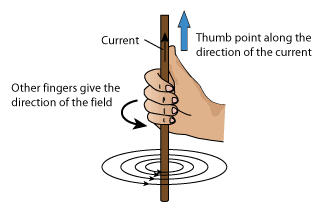
\includegraphics[width=6cm]{250-Revision/rhsl.png}
            \caption{Right Hand Screw Law to determine magnetic field of charged wire}
            \label{fig:RHSL}
        \end{figure}
        
        RHSL for determining charged solenoid wire $\overrightarrow{B}$ field: if the rest of four fingers are curled parallel to the current of wire, then the thumb pointing to the direction of $\overrightarrow{B}$ field.
        \item Fleming's Right Hand Rule or Left Open-handed Law for $\overrightarrow{F_B}$ direction:
            \subitem a) (Fig \ref{fig:lorentz-dir} left) Extend the thumb + first two fingers of right hand. The first finger points to $\overrightarrow{B}$ field direction and the thumb points to direction of $\overrightarrow{v}$ of positive charge (if it's electron then the $\overrightarrow{v}$ direction reversed). Then the second finger points to the direction of $\overrightarrow{F_B}$. This is \textit{Fleming's Right Hand Rule for Lorentz Force.}
            
            \subitem b) (Fig \ref{fig:lorentz-dir} right) Fully extend the left hand. Let the $\overrightarrow{B}$ field lines pass through the palm, while the four fingers points to the direction of $\overrightarrow{v}$ of positive charge, the thumb points to direction of $\overrightarrow{F_B}$. This is called \textit{Left Hand Rule for Lorentz Force}.
            \begin{figure}[ht]
                \centering
                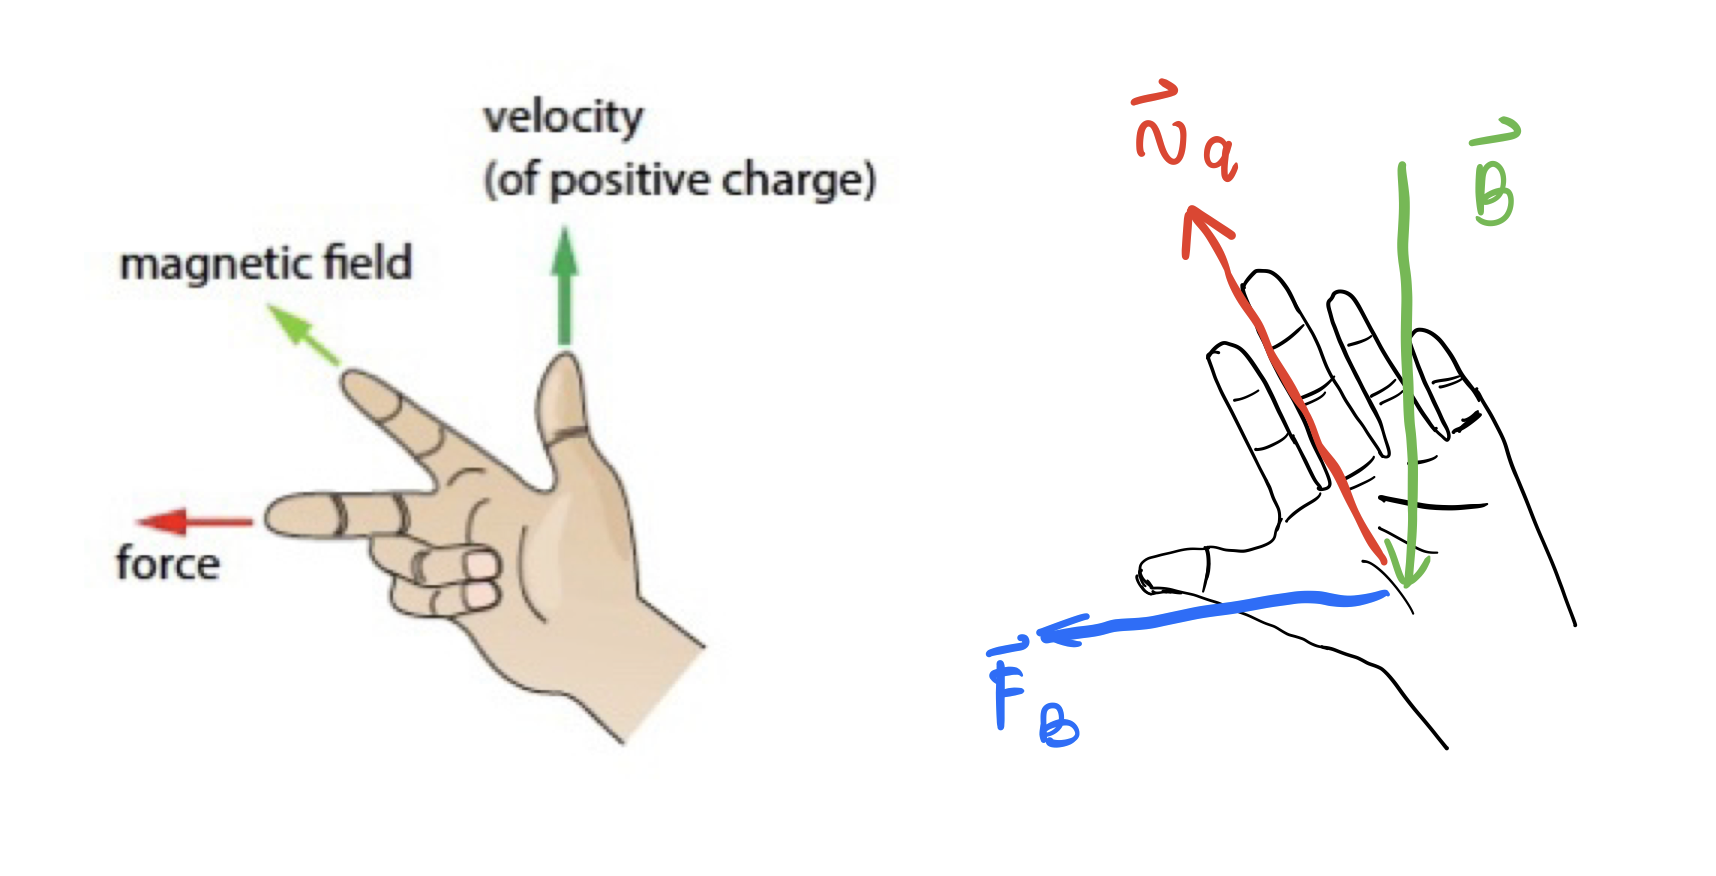
\includegraphics[width=12cm]{250-Revision/lorentz-force-dir.png}
                \caption{Two rules for determining the direction of Lorentz Force.}
                \label{fig:lorentz-dir}
            \end{figure}
        
    \end{itemize}
    If the $\overrightarrow{E}$ field also exists, then the net force (electric and magnetic) for the positively charged particle would be:
    \begin{equation}
        \overrightarrow{F}=q(\overrightarrow{E}+\overrightarrow{v}\times \overrightarrow{B})
    \end{equation}

\subsubsection{Cyclotron Motion Analysis}
    \begin{figure}[ht]
        \centering
        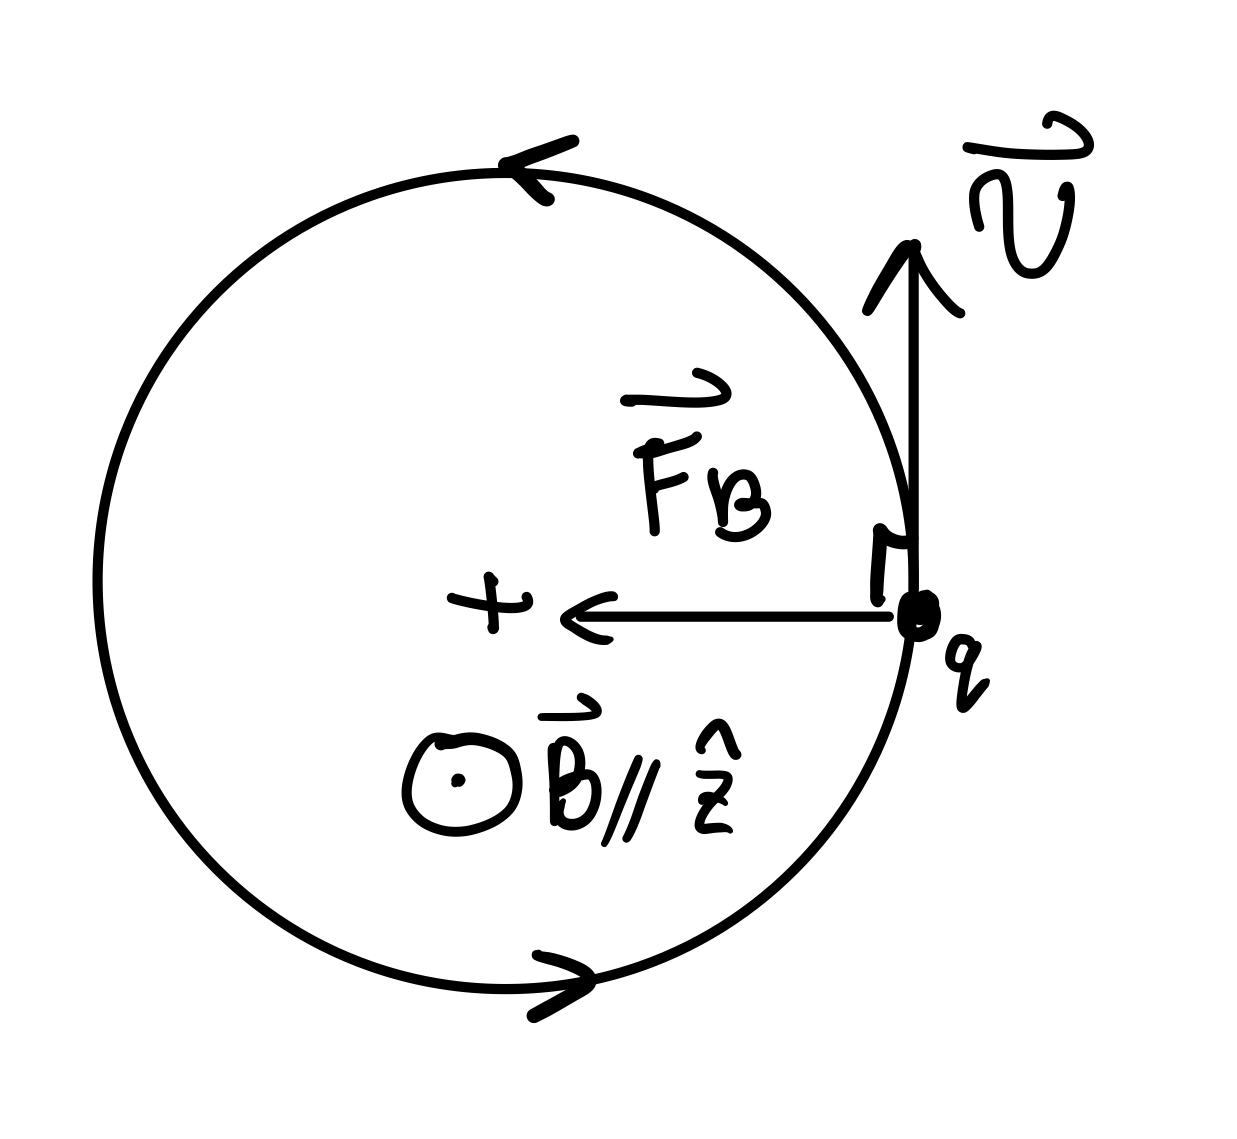
\includegraphics[width=5cm]{250-Revision/cyclotron.png}
        \caption{A cyclotron}
        \label{fig:cyclotron}
    \end{figure}
    
    \noindent Suppose we have a positive charge $Q$. We flick it with initial velocity $\overrightarrow{v}$ in the constant $\overrightarrow{B}$ field. Then this particle will rotate counterclockwise around a center with some distance $R$, and this charge is called \textit{cyclotron}.
    
    \begin{itemize}
        \item Direction of magnetic force?
        
        From Lorentz Law, and by using Fleming's LHR, as $\overrightarrow{B}$ lines comes out of the page, the magnetic force $\overrightarrow{F_B}$ is perpendicular to the velocity vector. Notice that $\overrightarrow{F_B}$ is centripetal force of the charge, allowing the charge to do circular motion.
        
        \item Velocities in polar/cylindrical coordinates...
        
        Since the charge is doing circular motion on the $xy$-plane, we can use cylindrical (polar) coordinates $(x,y,z)\to(s,\phi, z)$.
        
        Recall that, $\overrightarrow{B}=B\hat{z}$ and:
        \begin{eqnarray*}
            \overrightarrow{v} &=& \overrightarrow{r}'\\
                               &=& v_s\hat{s} + v_\phi\hat{\phi}+v_z\hat{z}\\
                               &=& 0 + R\dot{\phi}\hat{\phi}+\dot{z}\hat{z}
        \end{eqnarray*}
        \begin{equation*}
            \overrightarrow{a} = \underbrace{(\dot{\phi})^2R}_{a_s=v_\phi^2/R}\hat{s}+R\ddot{\phi}\hat{\phi}+\ddot{z}\hat{z}
        \end{equation*}
        
        Then:
        \[\overrightarrow{v}\times\overrightarrow{B}=\begin{bmatrix}0\\v_\phi  \\ \dot{z}\end{bmatrix}\times \begin{bmatrix}0\\0  \\B \end{bmatrix}=\begin{bmatrix}v_\phi B\\0  \\0 \end{bmatrix}\]
        \[\renewcommand\arraystretch{1.5}
        m\overrightarrow{a}=\begin{bmatrix}\frac{mv_\phi^2}{R}\\mR\ddot{\phi}  \\ m\ddot{z}\end{bmatrix}
        =\begin{bmatrix}Qv_\phi B\\0 \\0 \end{bmatrix}\]
        \[\implies
        \begin{cases}
            v_\phi^2m &= QBv_\phi R\\
            \ddot{\phi} &= 0\\
            \ddot{z} &= 0
        \end{cases}
        \]
        \[v_\phi = \frac{QBR}{m}\implies mv_\phi = p =QBR\]
        \[R = \left | \frac{mv_\phi}{QB} \right |\]
        \[T=\frac{2\pi R}{|v_\phi|}\implies \omega=\frac{2\pi}{T}=\frac{|QB|}{m}\]
        
    \item In the ocean... (Coriolis effects on ocean currents)
    \[\overrightarrow{a}=\overrightarrow{v}'=\frac{\overrightarrow{F_c}}{m}=-f(\overrightarrow{v}\times \hat{z})\]
    \[\omega = |f|=2\Omega|\sin(\phi)|\]
    \[R=\left|\frac{v}{f}\right|\]
    \end{itemize}
    \newpage
    
\subsubsection{Hall Effect: Measuring B field}
    \begin{figure}[ht]
        \centering
        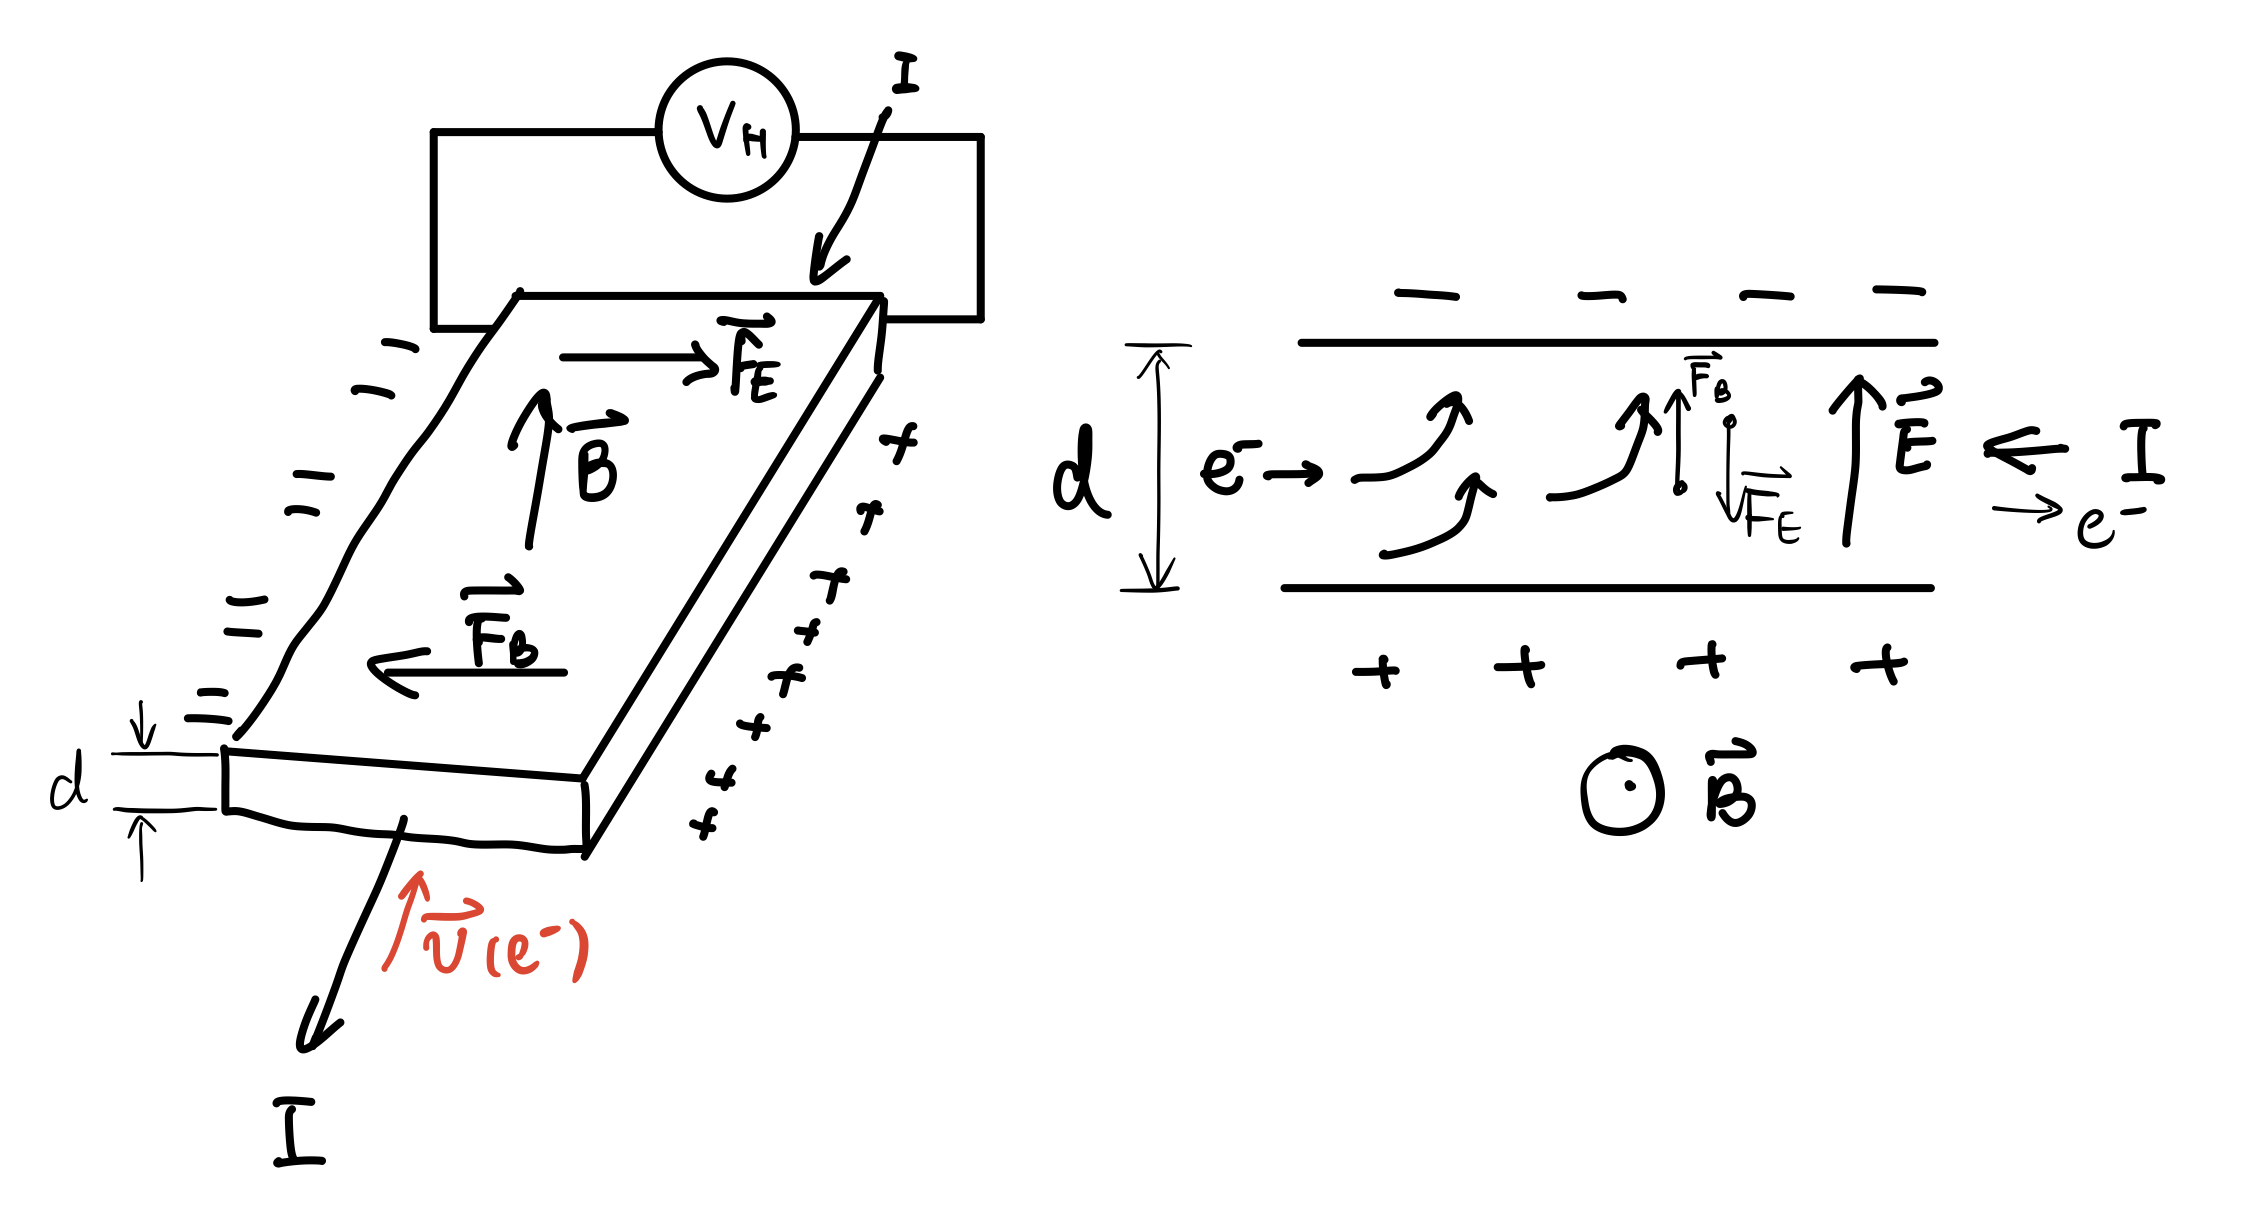
\includegraphics[width=12cm]{250-Revision/hall.png}
        \caption{The Hall Effect Schematics}
        \label{fig:hall-effect}
    \end{figure}
    
    \noindent Suppose we have a rectangular conductor with thickness $d$, if we impose a current $I$ on this conductor in a $\overrightarrow{B}$ field then we can indirectly evaluate the B field magnitude.
    \begin{itemize}
        \item At first, the conductor is electrically neutralized and its net charge is zero.
        \item When we impose current on this conductor, the electrons will move through the conductor, with opposite direction from the current direction.
        \item However, due to existence of $\overrightarrow{B}$ field, there exists Lorentz force on this electron, deflecting the motion path toward the boundary of conductor, accumulating on it.
        \item At this time, the opposite boundary, due to charge imbalance, will "accumulate" positive charges, forming $\overrightarrow{E}$ field.
        \item Now electrons have both $\overrightarrow{F_B}$ and $\overrightarrow{F_E}$, continuing piling up toward the boundary until the forces are balanced, i.e.
        \[||\overrightarrow{F_B}||=||\overrightarrow{F_E}||\]
        \[\cancel{Q}Bv=\cancel{Q}E=\frac{\cancel{Q}V}{d}\]
        \[B=\frac{V}{d\cdot v}\]
        where $Q=e$, $v$ is electron velocity magnitude, $V$ is electric potential (voltage), which can be directly measured through voltmeter.
    \end{itemize}

\subsubsection{Electric Current}
    \begin{description}
        \item[Definition] Electric current is amount of charge passing through point per unit time. Unit: Amp\`ere (A), 1A= 1C/s
    \end{description}
    The electric current requires continuous charge distribution, and we will analyze it by 3 cases.
    
    \begin{enumerate}
        \item 1D distribution
        
        \begin{figure}[t]
            \centering
            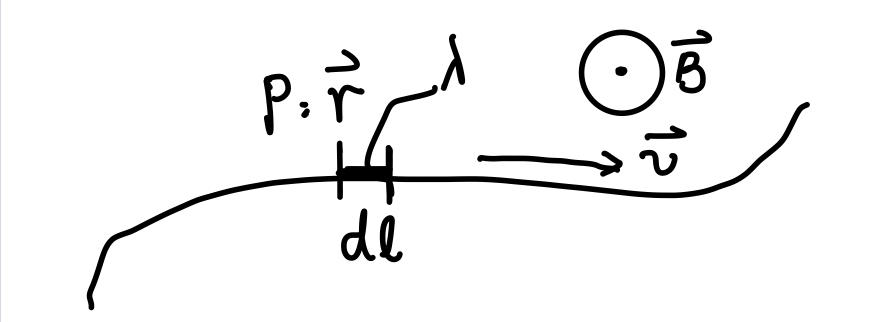
\includegraphics[width = 10cm]{250-Revision/current-1d.jpeg}
        \end{figure}
        
        We know the charge density $\lambda (\overrightarrow{r},t)$ of wire, and the charge moves at velocity $\overrightarrow{v}(\overrightarrow{r}, t)$.
        
        Then amount of charge, $dQ$, passing through point $P$ during infinitesimal time period $dt$ is:
        \[dQ=\lambda vdt\implies \boxed{I=\frac{dQ}{dt}=\lambda v}\]
        
        Now we introduce $\overrightarrow{B}$ field, then what will be the magnetic force $\overrightarrow{F_B}$? From Lorentz Force Law, $\overrightarrow{F_B}$ also applies for the infinitesimals:
        \[d\overrightarrow{F_B}=\lambda dl(\overrightarrow{v}\times \overrightarrow{B})\]
        \[\overrightarrow{F_B}=\int_{\mathcal{W}}\lambda dl(\overrightarrow{v}\times \overrightarrow{B})=\int_{\mathcal{W}}(\overrightarrow{I}\times \overrightarrow{B})dl\]
        Since $\overrightarrow{I}\parallel d\overrightarrow{l}$, we can move the vector arrow to another quantity:
        \[\overrightarrow{I}dl=Id\overrightarrow{l}\]
        Thus:
        \begin{equation}
            \boxed{\overrightarrow{F_B}=\int_{\mathcal{W}}I(d\overrightarrow{l}\times \overrightarrow{B})}
        \end{equation}
        where $\mathcal{W}$ is the whole wire.
        
        \item 2D charge density: \(\sigma\)
        \begin{figure}[ht]
            \centering
            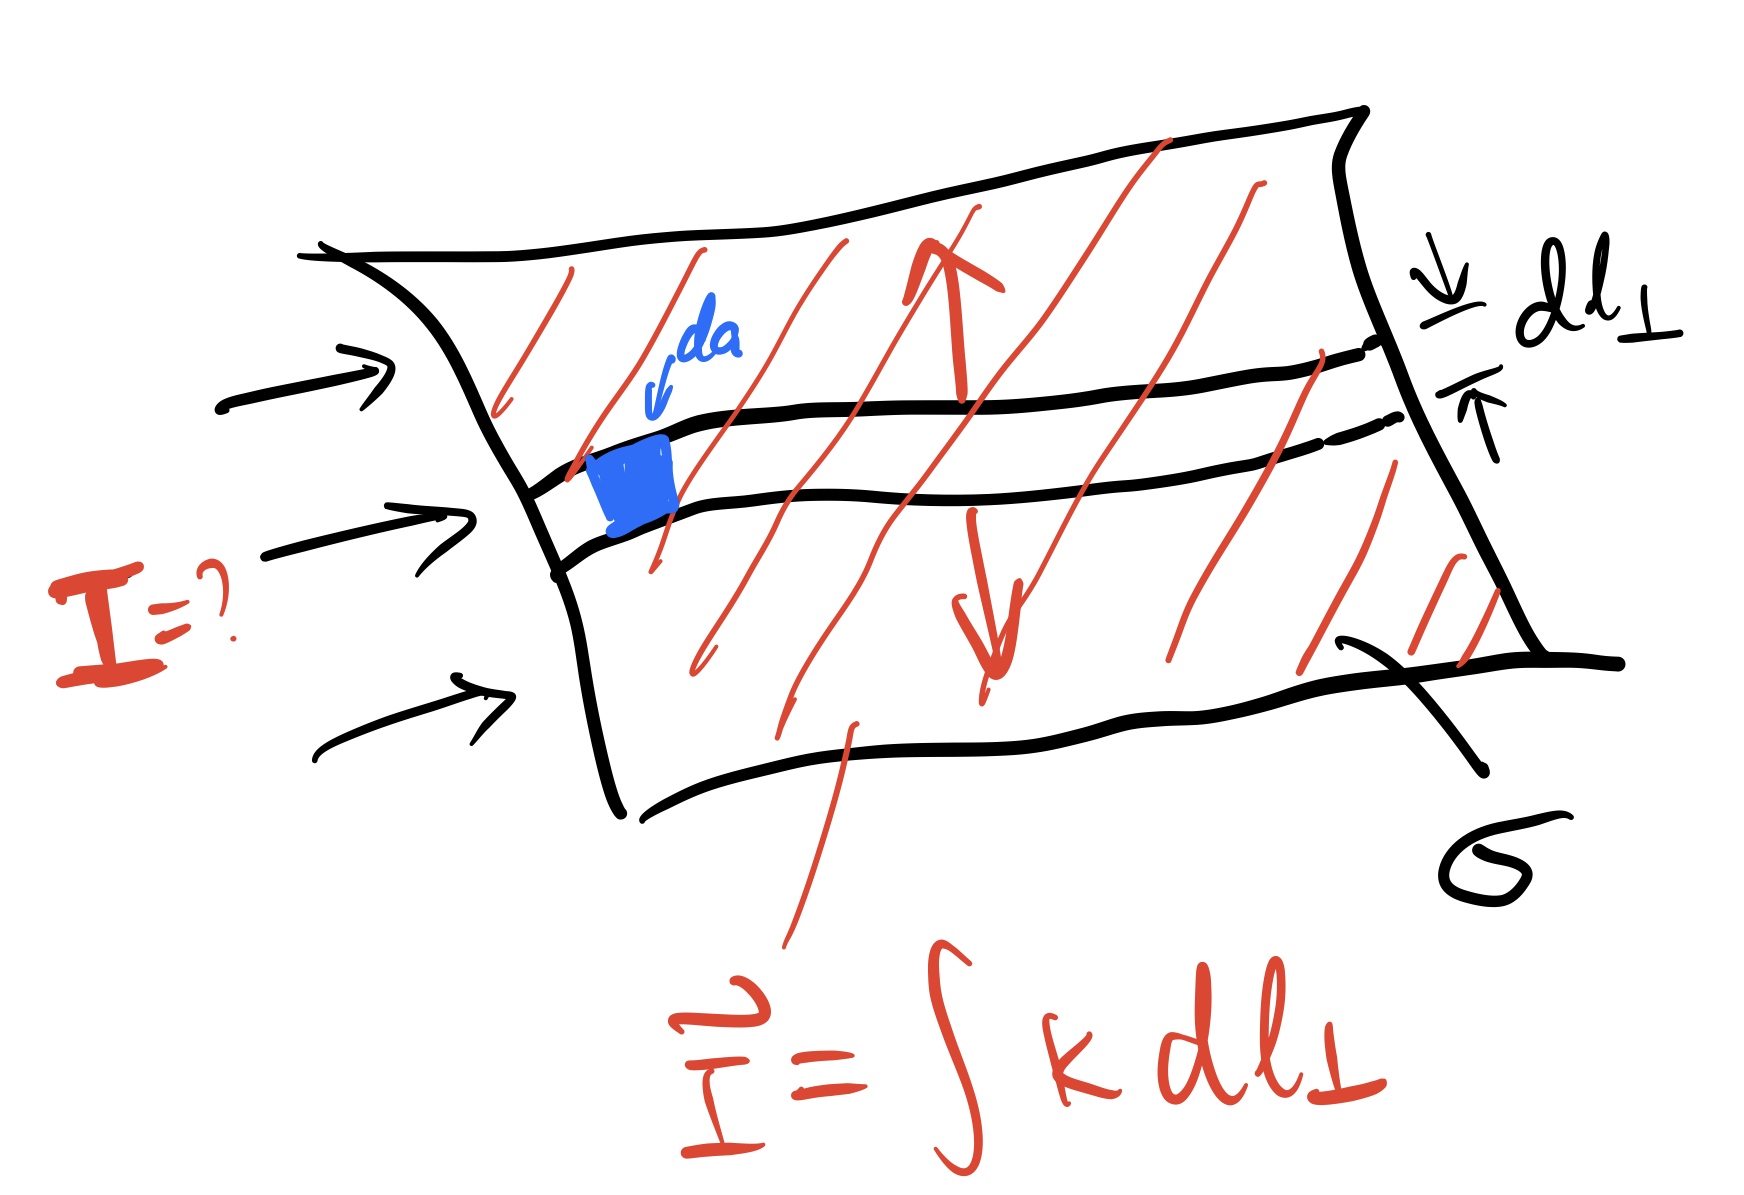
\includegraphics[width=8cm]{250-Revision/current-2d.jpeg}
        \end{figure}
        
        Intuitively, the current equals to $\sigma A$ where $A$ is area of this surface. The next step is to show this rigorously.
        
        We define a new variable $\overrightarrow{K}$, which is \textbf{surface current density}:
        \[\overrightarrow{K}=\sigma \overrightarrow{v}\]
        
        Then the electric current will be the integration of $\overrightarrow{K}$ over the width/height of surface:
        \begin{equation*}
            \boxed{\overrightarrow{I}=\int_{\mathrm{width}} \overrightarrow{K}dl_\perp}
        \end{equation*}
        
        Then what about $\overrightarrow{F_B}$?
        \[dQ=\sigma da\implies d\overrightarrow{F}=\sigma da(\overrightarrow{v}\times \overrightarrow{B})=\overrightarrow{K}\times \overrightarrow{B}da\]
        \begin{equation}
            \boxed{\overrightarrow{F_B} = \iint_{\mathcal{S}}(\overrightarrow{K}\times \overrightarrow{B})da}
        \end{equation}
        where $\mathcal{S}$ is the whole sheet of surface.
        
        \item 3D distribution: $\rho(\overrightarrow{r}, t)$
        \begin{figure}[ht]
            \centering
            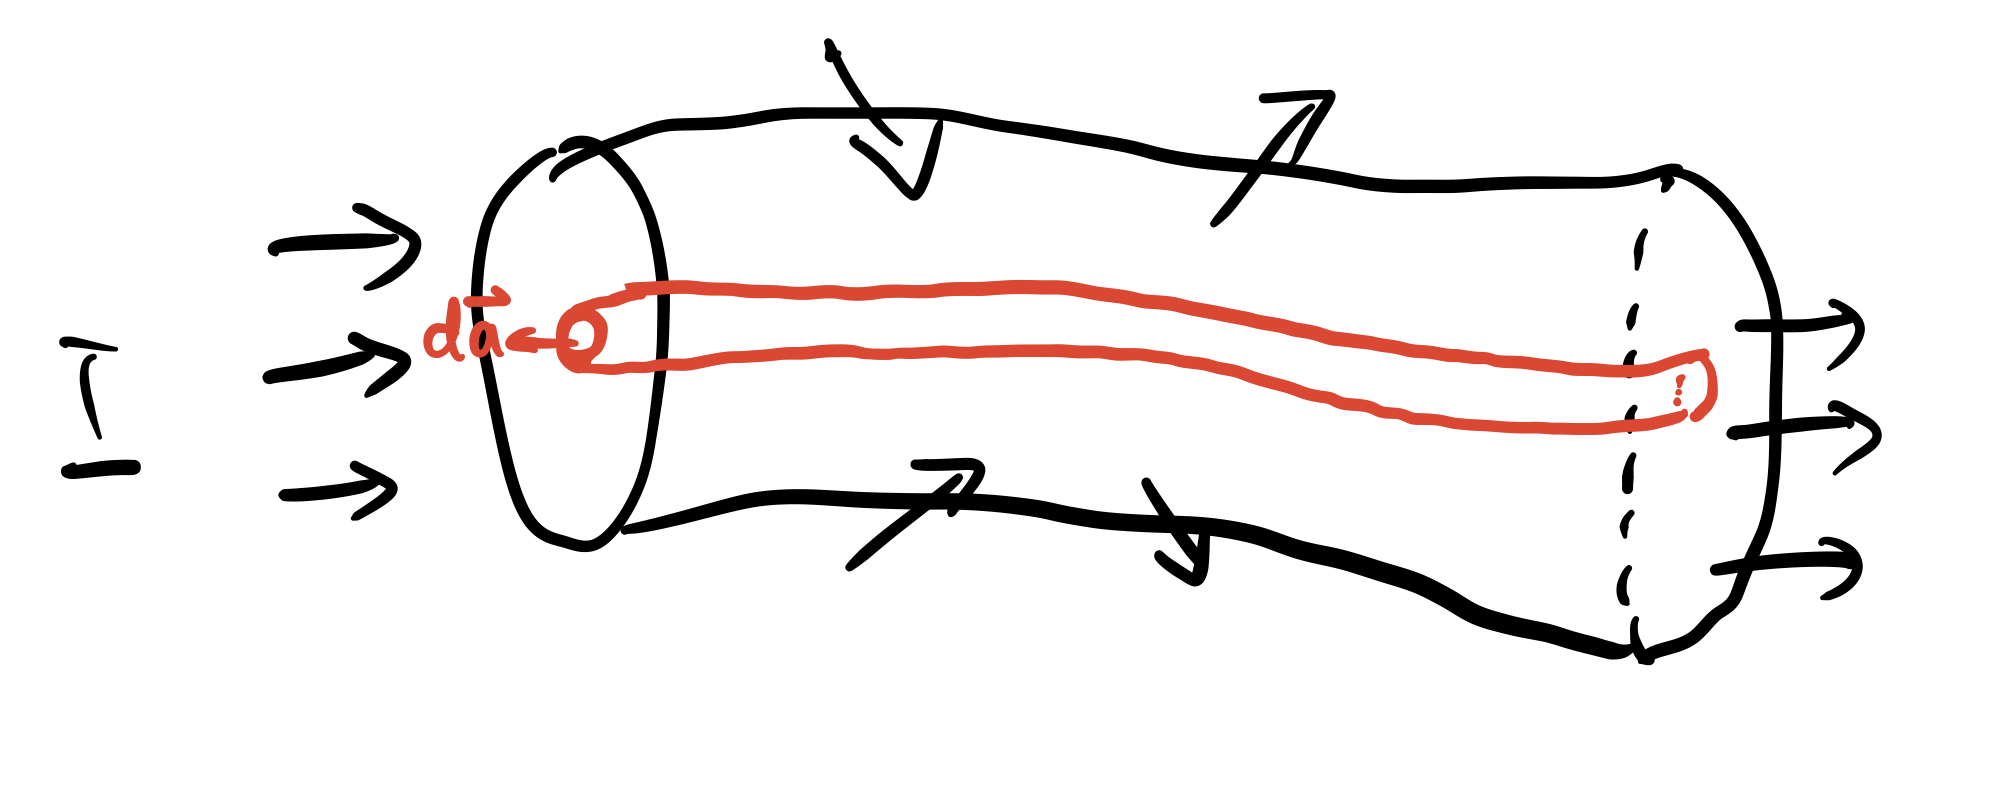
\includegraphics[width=8cm]{250-Revision/current-3d.png}
        \end{figure}
        
        Similar in 2D, we define \cancel{current change} volume current density $\overrightarrow{J}$:
        \[\overrightarrow{J}=\rho\overrightarrow{v}\]
        \[\implies \boxed{I=\iint_{\mathcal{S}_\mathrm{wire}}\overrightarrow{J}\cdot d\overrightarrow{a}}\]
        where $\mathcal{S_{\mathrm{wire}}}$ is the cross-section of wire.
        \[dQ=\rho d\tau\implies d\overrightarrow{F_B}=\rho d\tau(\overrightarrow{v}\times \overrightarrow{B})\]
        \begin{equation}
            \boxed{\overrightarrow{F_B}=\iiint_{\mathrm{wire}}\rho(\overrightarrow{v}\times \overrightarrow{b})d\tau=\iiint_{\mathrm{wire}}(\overrightarrow{J}\times \overrightarrow{B})d\tau}
        \end{equation}
    \end{enumerate}
    
    \noindent\textit{Example}\\
    \noindent We have an infinitely long wire with radius $R$ and volume current density
    \[\overrightarrow{J}=J_0\left(1-\frac{s^2}{R^2}\right)\hat{z}\]
    then what is $I$? (Cylindrical coordinates):
    
    \noindent \textit{Solution}
    \begin{eqnarray*}
        I = \iint_{\mathcal{S}}\overrightarrow{J}\cdot d\overrightarrow{a} &=& \int_{0}^{2\pi}d\phi\int_{0}^{R}J_0 sds\left(1-\frac{s^2}{R^2}\right)\\
        &=& 2\pi J_0\left[\frac{s^2}{2}-\frac{s^4}{4R^2}\right]^{R}_{0}\\
        &=& \frac{\pi J_0 R^2}{2}
    \end{eqnarray*}
    
\subsubsection{Charge Conservation Law and Continuity Equation}
Suppose we have a solid sphere $\mathcal{V}$, with some volume charge density $\overrightarrow{J}$, and some enclosed charge $Q_{\mathrm{enc}}$. Then what will be the current of this sphere?\\

\noindent From Electrostatics regime:
\[Q_{\mathrm{enc}}=\iiint_{\mathcal{V}} \rho d\tau\]
And from definition of electric current, in the Magnetostatic regime:
\begin{eqnarray*}
I &=& \frac{dQ_{\mathrm{enc}}}{dt}\\
&=&\frac{d}{dt}\iiint_\mathcal{V} \rho(\overrightarrow{r}, t) d\tau\\
&=&\iiint_\mathcal{V}\frac{\partial \rho}{\partial t}d\tau\\
&=& 0
\end{eqnarray*}

\noindent We have known that, the charge "flow" $dI$ is defined by:
\[dI=\rho\overrightarrow{v}\cdot d\overrightarrow{a}\]
Then the charge crossing the surface $\mathcal{S}$ is:
\[I=\iint_\mathcal{S}\overrightarrow{J}\cdot d\overrightarrow{a}\]
If the solid $\mathcal{V}$ consists of a whole surface, then the charge per unit time flowing through this solid will be:
\[\oiint_{\mathcal{S}}\overrightarrow{J}\cdot d\overrightarrow{a}\]
Note that if $\oiint<0$, then the charges will accumulate in solid $\mathcal{V}$. If $\oiint>0$, then the charges will leave this solid. And also notice that, this will also lead to change in enclosed charge $Q_{\mathrm{enc}}$, according to the law of conservation of charges:\
\begin{description}
    \item[Law of Charge Conservation] Charges are never formed or extinguished, and there only exists the charge movement. That is, there is no "source" emitting charges or "sink" absorbing charge inside solid $\mathcal{V}$. If this solid accumulates charges, then there must be change in enclosed charge $Q_{\mathrm{enc}}$.
\end{description}

\noindent This implies that:
\begin{equation*}
    \frac{dQ_{\mathrm{enc}}}{dt}=\boxed{\iiint_{\mathcal{V}} \frac{\partial \rho}{\partial t}d\tau=-\oiint_{\mathcal{S}}\overrightarrow{J}\cdot d\overrightarrow{a}}
\end{equation*}
By applying Green's Theorem:
\[\oiint_{\mathcal{S}} \overrightarrow{J}\cdot d\overrightarrow{a}=\iiint_\mathcal{V}(\nabla\cdot \overrightarrow{J})d\tau\implies -\iiint_{\mathcal{V}} \frac{\partial \rho}{\partial t}d\tau=\iiint_\mathcal{V}(\overrightarrow{\nabla}\cdot \overrightarrow{J})d\tau\]
Then:
\begin{equation}
    \boxed{
    \overrightarrow{\nabla} \cdot \overrightarrow{J} = -\frac{\partial \rho}{\partial t}
    }
    \label{eq: Continuity equation}
\end{equation}
This is called the \textbf{continuity equation}, and is precise math statement of local charge conservation. And in MAGNETOSTATIC regime:
\[\overrightarrow{\nabla} \cdot \overrightarrow{J} = -\frac{\partial \rho}{\partial t}=0\]
This is also the condition of being magnetostatic.

\subsection{Biot-Savart Law}
We have known that, by using the right hand screw law, the $\overrightarrow{B}$ field lines of a straight line current are like some "concentric circles" curling around the wire. This is a \textit{qualitative} statement, and in this section we are going to analyze the magnetic field \textit{quantitatively}.\\

\noindent Lorentz force law gives the magnetic force on current when there exists a magnetic field. And we also know that current creates magnetic field, which is concluded by \textbf{Biot-Savart Law}:

\begin{equation}
    \boxed{
    \overrightarrow{B} = \frac{\mu_0}{4\pi}\int_{\mathcal{W}}\frac{\overrightarrow{I}\times \hrc}{\rc^2}dl=\frac{\mu_0I}{4\pi}\int_{\mathcal{W}}\frac{d\overrightarrow{l}\times \hrc}{\rc^2}
    }
    \label{Eq: Biot-Savart}
\end{equation}
where $\mu_0=4\pi\times 10^{-7}$ N A$^{-2}$, the vacuum permeability. The unit of $\overrightarrow{B}$ field is Tesla (T). Tesla is a very large unit, and in regular physics lab the B field strength is usually $5\times 10^{-5}$ T, or 0.5 Gauss.


\subsection{Divergence and Curl of Magnetic Field}
\subsection{Magnetic Vector Potential}
\section{Electrodynamics}
\subsection{Electromotive Force}
\subsection{Electromagnetic Induction}
\subsection{Maxwell's Equations}

\end{document}
